\documentclass[a4paper,11pt]{article}
\usepackage[T1]{fontenc}
\usepackage[utf8]{inputenc}
\usepackage{graphicx}
\usepackage{xcolor}


\usepackage{amsmath,amssymb,amsthm,textcomp}
\usepackage{enumerate}
\usepackage{multicol}
\usepackage{tikz}
\usepackage[english, russian]{babel}

\usepackage{geometry}
\geometry{total={210mm,297mm},
	left=25mm,right=25mm,%
	bindingoffset=0mm, top=20mm,bottom=20mm}


% custom footers and headers
\usepackage{fancyhdr}
\pagestyle{fancy}
\lhead{}
\chead{}
\rhead{}
\lfoot{}
\cfoot{}
\rfoot{}
\renewcommand{\headrulewidth}{0pt}
\renewcommand{\footrulewidth}{0pt}

%%%----------%%%----------%%%----------%%%----------%%%

\begin{document}
\textbf{\large Задача 1}
\medskip\hrule\medskip
\textsl{Пользуясь правилом Лопиталя, найдите пределы. (4) }
\begin{align*}
	\textsl{(a)} & \lim_{x \to 0} \frac{(x + 1) \sin x^2}{x^2 e^x} \\
	\textsl{(б)} & \lim_{x \to +\infty} (\sqrt{x} - \ln x) \\
	\textsl{(в)} & \lim_{x \to +\infty} x^{\arctan(1/x)}
\end{align*} \\
\noindent
a)
\begin{gather*}
	\lim_{x \to 0} \frac{(x + 1) \sin x^2}{x^2 e^x} =  
	\lim_{x \to 0} \frac{x + 1}{e^{x}} \cdot \lim_{x \to 0} \frac{\sin x}{x} = \lim_{x \to 0} \frac{ 1}{e^{x}} \cdot \lim_{x \to 0} \frac{\cos x}{1} = 1	
\end{gather*}


\noindent
б)
\begin{gather*}
	\lim_{x \to +\infty} (\sqrt{x} - \ln x) =  	
	\lim_{x \to +\infty} (\ln e^{\sqrt{x}} - \ln x) = 
	\lim_{x \to +\infty} (\ln \dfrac{e^{\sqrt{x}}}{x}) =  \\
	\textit{ = | в силу непрерывности логарифма | = } \\
	= \ln (\lim_{x \to +\infty} \dfrac{e^{\sqrt{x}}}{x})   
	= \ln (\lim_{x \to +\infty} \frac{(\frac{e^{\sqrt{x}}}{2\sqrt{x}})}{1}) = 
	\ln (\lim_{x \to +\infty} \frac{e^{\sqrt{x}}}{2\sqrt{x}}) = \infty
\end{gather*}

\noindent
в)
\begin{gather*}
	\lim_{x \to +\infty} x^{\arctan(1/x)} = 	
	\lim_{x \to +\infty} e^{\ln x \arctan(1/x)} = 	
	\lim_{x \to +\infty} e^{\dfrac{\arctan(1/x)}{1/\ln x}} = \\
	\textit{ = | в силу непрерывности экспоненты | = } \\
	= e^{\lim_{x \to +\infty} \dfrac{\arctan(1/x)}{1/\ln x}} = 
	e^{\lim_{x \to +\infty} \dfrac{\dfrac{1}{1 + (\frac{1}{x})^2} \cdot (- \frac{1}{x^2ь})}{(-\frac{1}{\ln^2 x}) \cdot \frac{1}{x}}} = 
	e^{\lim_{x \to +\infty} \dfrac{x \ln^2 x }{x^2 + 1}} = \\
	= e^{\lim_{x \to +\infty} \dfrac{\frac{\ln^2 x}{x} }{1 + \frac{1}{x^2}}} = 
	e^{0} = 1
\end{gather*}
\newpage



%%%----------%%%----------%%%----------%%%----------%%%






\textbf{\large Задача 2}
\medskip\hrule\medskip
\textsl{Представьте формулой Тейлора с $ o((x - x_0)^3) $  в окресности точки $ x_0 $ функцию $ f(x) $. (8)}
\begin{align*}
	f(x) = \ln \frac{1 + x}{2 - x}, \qquad x_0 = 1
\end{align*} \\
 
Сделаем замену $ x = x_0 + t = 1 + t $. Тогда наша функция примет вид:
\begin{gather*}
	f(x) = \ln \frac{1 + x}{2 - x} = 
	\ln \frac{2 + t}{1 - t} = 
	\ln (2 + t) - \ln (1 - t) = 
	\ln 2(1 + \frac{t}{2}) - \ln (1 - t) = 
	\begin{bmatrix}
	 a = \dfrac{t}{2} \\[5pt]
	 b = (-t) 
	\end{bmatrix} = \\
	= \ln 2 + \ln (1 + a) - \ln (1 + b) = 
	\ln 2 + (1 + a - \frac{a^2}{2} + \frac{a^3}{3} + o(a^3)) - (1 + b - \frac{b^2}{2} + \frac{b^3}{3} + o(b^3)) = \\
	= \ln 2 + (a - b) - \frac{a^2 - b^2}{2} + \frac{a^3 - b^3}{3} + o(a^3) + o(b^3) = 
	\ln 2 + \frac{3t}{2} + \frac{3t^2}{8} + \frac{3t^3}{8} + o(t^3)  = \\
	= \ln 2 + \frac{3(x - x_0)}{2} + \frac{3(x - x_0)^2}{8} + \frac{3(x - x_0)^3}{8} + o((x - x_0)^3)	
\end{gather*} 
\\ \\ \\


%%%----------%%%----------%%%----------%%%----------%%%







\textbf{\large Задача 3}
\medskip\hrule\medskip
\textsl{Представьте формулой Тейлора с $ o((x - x_0)^n) $ в окресности точки $ x_0 $ функцию $ f(x) $, используя разложения основных элементаных функций.(12)}
\begin{align*}
	f(x) = \sqrt[3]{8 - x^3}, \qquad x_0 = 0
\end{align*} \\

Произведем замену $ t = -(\frac{x - x_0}{2})^3 = -(\frac{x}{2})^3$. Тогда наша функция примет вид:
\begin{gather*}	
	f(x) = \sqrt[3]{8 - x^3} = 
	2 \sqrt[3]{1 + t} = 
	2\begin{bmatrix}(1 + \sum\limits_{k = 1}^{\infty} \dbinom{1/3}{k}t^k)\end{bmatrix} = \\
	= 2\begin{bmatrix}(1 + \sum\limits_{k = 1}^{\lceil \frac{n}{3}\rceil} \dbinom{1/3}{k} \frac{(-1)^k \cdot (x - x_0)^{3k} }{2^{3k}}) + o((x - x_0)^n) \end{bmatrix} = \\
	= 2 + \sum\limits_{k = 1}^{\lceil \frac{n}{3}\rceil} \dbinom{1/3}{k} \frac{(-1)^k \cdot (x - x_0)^{3k} }{2^{3k} /2}) + o((x - x_0)^n)  
\end{gather*}
\text{Как подсказал семинарист, этого достаточно :)}
\newpage



%%%----------%%%----------%%%----------%%%----------%%%







\textbf{\large Задача 4}
\medskip\hrule\medskip
\textsl{С помощью формулы Тейлора  найдите приближенное значение числа с точностью до $ 0, 001 $.(16)} 
\begin{align*}
	\sqrt{1.5}
\end{align*} \\

Воспользуемся разложением уже известной базовой функции, с остаточным членом в виде Лагранжа:  
\begin{gather*}
	f(x) = \sqrt{1 + x} =
	\sum_{i = 0}^{n} \frac{(-1)^n (2n!)}{(1 - 2n)(n!)^2(4^n)}x^n + \frac{(-1)^{n + 1} ((2n + 2)!)}{(-1 - 2n)((n + 1)!)^2(4^{n + 1})} \cdot \frac{\epsilon^{n + 1}}{(1 + \epsilon)^{\frac{2n + 1}2}}
\end{gather*}
Рассмотрим отношение двух соседних членов этой суммы:
\begin{gather*}
\frac{(-1)^{n + 1} ((2n + 2)!)}{(-1 - 2n)((n + 1)!)^2(4^{n + 1})}x^{n + 1} \; \div \; \frac{(-1)^n (2n!)}{(1 - 2n)(n!)^2(4^n)}x^n =\\[2pt]
= - \frac{(2n + 1)(2n + 2)(2n - 1)}{4(2n + 1)(n + 1)^2}x
= - \frac{(2n - 1)}{2(n + 1)}x < 1 \text{ поэтому наши слагаемые монотонно убывают}
\end{gather*}
Оценим остаточный член для $ n = 5 $
\begin{gather*}
\frac{(-1)^{n + 1} ((2n + 2)!)}{(-1 - 2n)((n + 1)!)^2(4^{n + 1})}\cdot \frac{\epsilon^{n + 1}}{(1 + \epsilon)^{\frac{2n + 1}2}} < 
\frac{(-1)^{n + 1} ((2n + 2)!)}{(-1 - 2n)((n + 1)!)^2(4^{n + 1})}x^{n + 1} = -\frac{21x^6}{1024} \approx 0.00032043 < 0.001
\end{gather*}
Таким образом, для того, чтобы получить необходимую точность, нам нужно выписать всего $ n = 5 $ слагаемых
\begin{gather*}
	f(x) = 1 + \frac{x}{2} - \frac{x^2}{8} + \frac{x^3}{16} - \frac{5x^4}{128} + \frac{7x^5}{256}
	= 1.22498 \approx 1,225
\end{gather*}
Стоит отметить, что в действительности $ \sqrt{1,5} $ равен $ 1,2247... \approx 1, 225$, что безусловно совпадает с полученным результатом. 
\\ \\



%%%----------%%%----------%%%----------%%%----------%%%



\textbf{\large Задача 5}
\medskip\hrule\medskip
\textsl{Вычислите предел с помощью формулы Тейлора. (20)}
\begin{align*}
	\lim_{x \to 0} \frac{x^2 e^x - \sqrt[3]{x^3 - 5x^2}}{\ln^2 (1 - x^3)}
\end{align*} \\

\begin{gather*}
	\lim_{x \to 0} \frac{x^2 e^x - \sqrt[3]{x^3 - 5x^2}}{\ln^2 (1 - x^3)} = 
	\lim_{x \to 0} \frac{x^2 (1 + o(1)) - \sqrt[3]{-5x^2 + o(x^2)}}{(x^3 + o(x^3))^2} = \\[2pt]
	= \lim_{x \to 0} \frac{x^2 + \sqrt[3]{5}x^{\frac{2}{3}} + o(x^{\frac{2}{3}})} {(x^6 + o(x^6))} = 
	\lim_{x \to 0} \frac{\sqrt[3]{5}x^{\frac{2}{3}} + o(x^{\frac{2}{3}})} {x^6} =
	\infty
\end{gather*}
\newpage





%%%----------%%%----------%%%----------%%%----------%%%





\textbf{\large Задача 6}
\medskip\hrule\medskip
\textsl{Для заданной функции $ f(x) = x^4 + 4x^3 - 2x^2 - 12x + 2 $ и отрезка $ [-2; 2] $ найдите:}
\begin{align*}
	& \textsl{а) промежутки возрастания и убывания, точки экстремума;} \\
	& \textsl{б) промежутки выпуклости и вогнутости, точки перегиба;} \\
	& \textsl{в) наибольшее и наименьшее значение функции на промежутке $ [-2; 2] $;}
\end{align*} \\

\begin{center}
	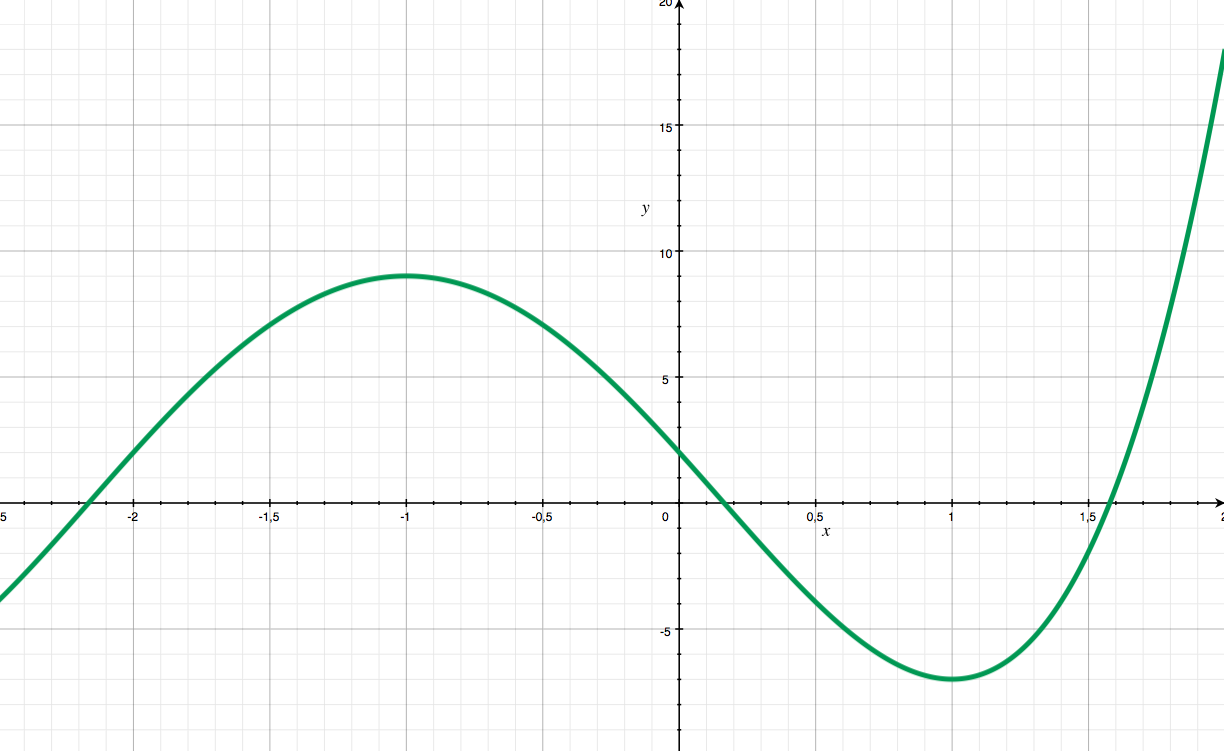
\includegraphics[width = 110mm]{images/61.png}	
\end{center}
\textsl{a)} Для этого пункта нам понадобиться первая производная:
\begin{gather*}
	f'(x) = 4x^3 + 12x^2 - 4x - 12 = 4(x^3 + 3x^2 - x - 3) = 4(x - 1)(x^2 + 4x + 3) = \\
	= 4(x - 1)(x + 1)(x+3)
\end{gather*} 
\begin{center}
	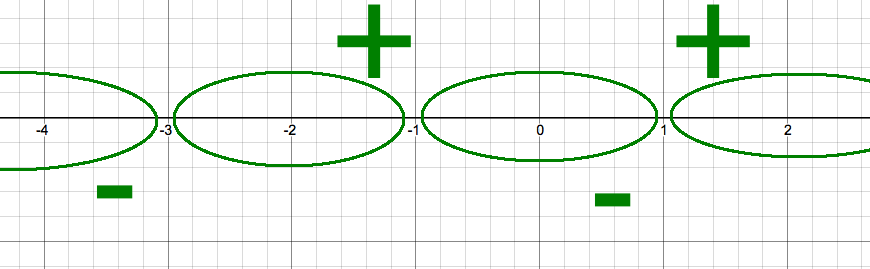
\includegraphics[width = 70mm]{images/62.png}
\end{center}
\noindent Промежутки возрастания функции   $\Longleftrightarrow f'(x) > 0 $:
\begin{gather*}
	x = (-2, -1) \cup (1, 2)
\end{gather*}

\noindent Промежутки убывания функции   $\Longleftrightarrow f'(x) < 0 $:
\begin{gather*}
x = (-1, 1)
\end{gather*}

\noindent Точки экстремума   $\Longleftrightarrow f'(x) = 0 $:
\begin{align*}
x &= -1 \quad y = 9 \\
x &= 1  \quad y = -7 
\end{align*}

\textsl{б)} Для поиска точек выпуклости и вогнутости необходимо исследовать второю производную:
\begin{gather*}	
	f''(x) = (f'(x))' = 4(3x^2 + 6x - 1) = 12(x + 1 + \frac{2}{\sqrt{3}})(x + 1 - \frac{2}{\sqrt{3}})
\end{gather*}


\begin{center}
	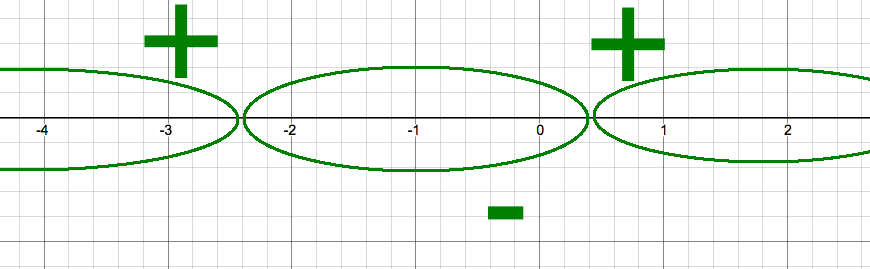
\includegraphics[width = 70mm]{images/63.png}
\end{center}
\noindent Промежутки  выпуклости вниз $\Longleftrightarrow f''(x) > 0 $:
\begin{gather*}
x = (\frac{2}{\sqrt{3}} - 1, 2)
\end{gather*}

\noindent Промежутки  выпуклости вверх $\Longleftrightarrow f''(x) < 0 $:
\begin{gather*}
x = (-2, \frac{2}{\sqrt{3}} - 1)
\end{gather*}

\noindent Точки перегиба   $\Longleftrightarrow f''(x) = 0 $:
\begin{align*}
x &= \frac{2}{\sqrt{3}} - 1 \quad y = \frac{1}{9} \\
\end{align*}

\textsl{в)} Для нахождения максимума мы должны сравнить значения функции в точках локального максимума и на концах интервала:
\begin{align*}
x &= -2 \quad y = 2 \\
x &= -1 \quad y = 9 \\
x &= 1 \quad y = -7 \\
x &= 2 \quad y = 18
\end{align*}
Отсюда $ max(f(x))  $ на промежутке $ [-2, 2] $ равен $ 18 $.
\newpage





%%%----------%%%----------%%%----------%%%----------%%%




\textbf{\large Задача 7}
\medskip\hrule\medskip
\textsl{Исследуйте функцию с помощью производных первого и второго порядка, постройте эскиз ее графика(28):}
\begin{align*}
	\textsl{a) }& y = \frac{-2x^3}{x^2 - 2x \pm 8}(-1)^n \\
	\textsl{б) }& y = e^{\frac{1}{x^2 - 2x \pm 8}}
\end{align*}
\textit{$ n $ - номер моего варианта $ \Rightarrow n = 4 \Rightarrow (-1)^n = 1$} \\
\\
1)
\begin{align*}
	y = \frac{-2x^3}{x^2 - 2x + 8}
\end{align*}
\begin{center}
	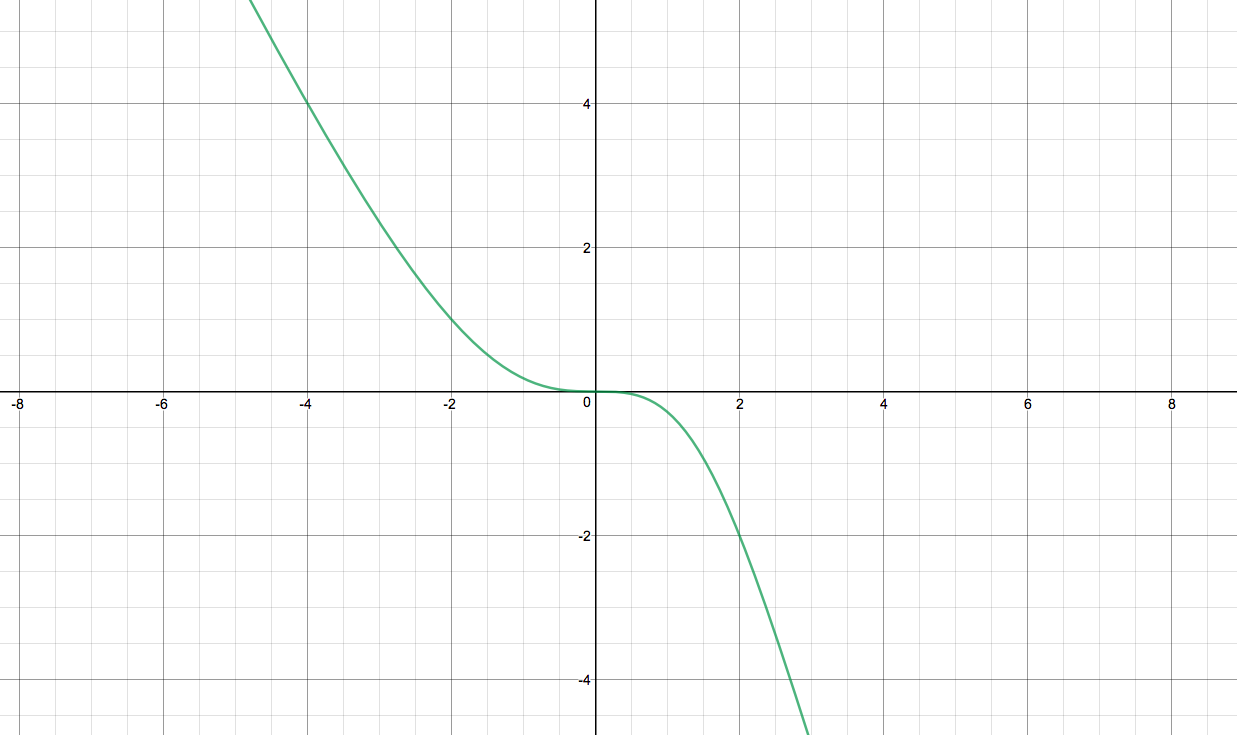
\includegraphics[width = 150mm]{images/711.png}
\end{center}

\noindent \textsl{1) ОДЗ:}
\begin{gather*}
x^2 - 2x + 8 \neq 0 \Rightarrow x - \textit{любое}
\end{gather*}

\noindent  \textsl{2) Первая производная:}
\begin{gather*}
f'(x) = \frac{-6x^2(x^2 - 2x + 8) - (-2x^3)(2x - 2)}{(x^2 - 2x + 8)^2} = \frac{-2x^2(x^2 - 4x + 24)}{(x^2 - 2x + 8)^2} \leq 0
\end{gather*} 
\begin{center}
	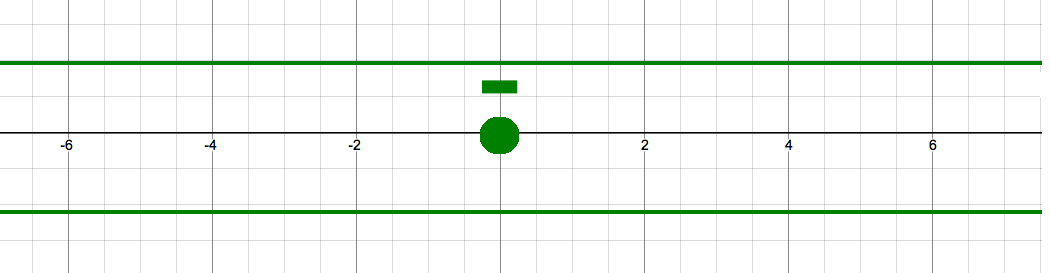
\includegraphics[width = 70mm]{images/712.png}
\end{center}

\noindent \textsl{3) Промежутки возрастания функции   $\Longleftrightarrow f'(x) > 0 $:}
\begin{gather*}
\cdots
\end{gather*}

\noindent \textsl{4) Промежутки убывания функции   $\Longleftrightarrow f'(x) < 0 $:}
\begin{gather*}
x \neq 0
\end{gather*}

\noindent \textsl{5) Точки экстремума   $\Longleftrightarrow f'(x) = 0 $:}
\begin{align*}
x = 0
\end{align*}

\noindent \textsl{6) Точки разрыва $ \Longleftrightarrow f'(x) $  - не определена:}
\begin{align*}
\cdots
\end{align*}

\noindent \textsl{7) Вторая производная:}
\begin{gather*}	
f''(x) = \frac{(-4x(x^2 - 4x + 24) - 2x^2(2x - 4))(x^2 - 2x + 8)^2 + 2x^2(x^2 - 4x + 24) \cdot 4(x - 1)(x^2 - 2x + 8) }{(x^2 - 2x + 8)^4} = \\
= \frac{16x(x^2 + 12x - 48)}{(x^2 - 2x + 8)^3} = \frac{16x(x - 2( \sqrt{21} - 3))(x - 2( - \sqrt{21} - 3))}{(x^2 - 2x + 8)^3}
\end{gather*}

\begin{center}
	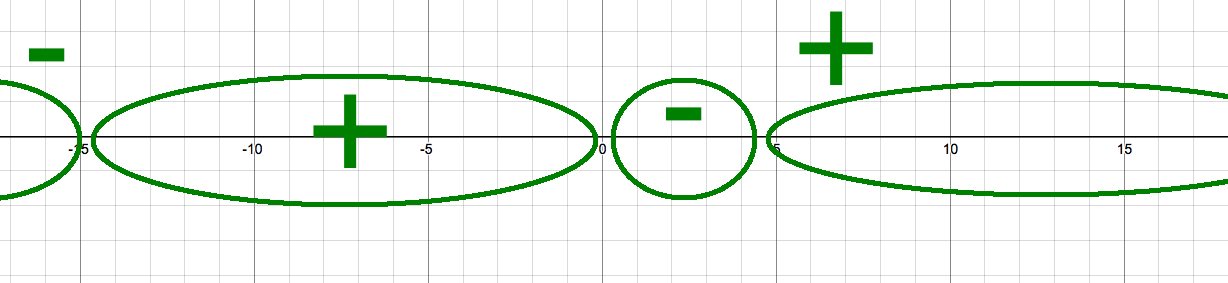
\includegraphics[width = 70mm]{images/713.png}
\end{center}
\noindent \textsl{8) Промежутки  выпуклости вниз $\Longleftrightarrow f''(x) > 0 $:}
\begin{gather*}
x = (2(-3 - \sqrt{21}), 0) \cup (2(\sqrt{21} - 3), \infty)
\end{gather*}

\noindent \textsl{9) Промежутки  выпуклости вверх $\Longleftrightarrow f''(x) < 0 $:}
\begin{gather*}
x = (-\infty, 2(-3 - \sqrt{21})) \cup (0, 2(\sqrt{21} - 3)) 
\end{gather*}

\noindent \textsl{10) Точки перегиба   $\Longleftrightarrow f''(x) = 0 $:}
\begin{align*}
x &= 0 \\
x &= 2(- \sqrt{21} - 3) \\
x &= 2(\sqrt{21} - 3) 
\end{align*}
\noindent \textsl{11) Ассимтоты:}
\begin{gather*}
k_1 = \lim_{x \to +\infty} \frac{f(x)}{x} = \frac{-2x^2}{x^2 - 2x + 8} = -2 \\
b_1 = \lim_{x \to +\infty} f(x) - kx = \frac{-2x^3}{x^2 - 2x + 8} + 2x = 
\frac{-2x^3 + 2x^3 - 4x^2 + 16x}{x^2 - 2x + 8} = \frac{- 4x^2 + 16x}{x^2 - 2x + 8} = -4 \\
\Rightarrow x \to -\infty: f(x) \to -2x - 4 \\ \\
k_2 = \lim_{x \to -\infty} \frac{f(x)}{x} = \frac{-2x^2}{x^2 - 2x + 8} = -2 \\
b_2 = \lim_{x \to +\infty} f(x) - kx = \frac{-2x^3}{x^2 - 2x + 8} + 2x = 
\frac{-2x^3 + 2x^3 - 4x^2 + 16x}{x^2 - 2x + 8} = \frac{- 4x^2 + 16x}{x^2 - 2x + 8} = -4 \\
\Rightarrow x \to -\infty: f(x) \to -2x - 4 
\end{gather*}
\newpage


2)
\begin{align*}
y = \frac{-2x^3}{x^2 - 2x - 8}
\end{align*}
\begin{center}
	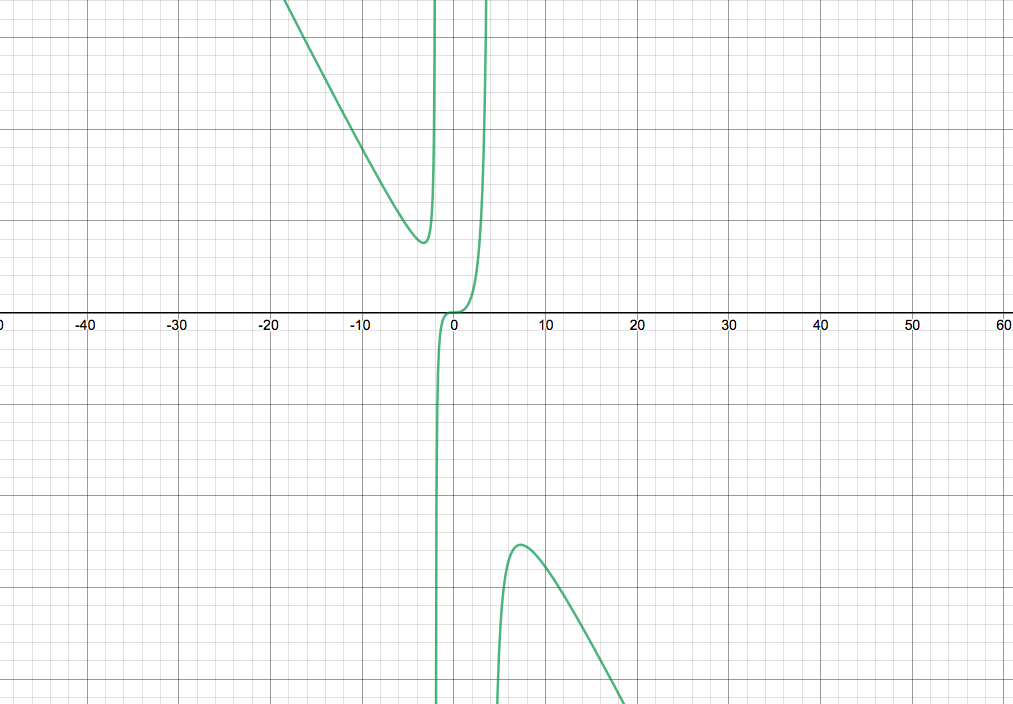
\includegraphics[width = 150mm]{images/721.png}
\end{center}

\noindent \textsl{1) ОДЗ:}
\begin{gather*}
x^2 - 2x - 8 \neq 0 \Rightarrow x \neq -2, 4
\end{gather*}

\noindent  \textsl{2) Первая производная:}
\begin{gather*}
f'(x) = \frac{-6x^2(x^2 - 2x - 8) - (-2x^3)(2x - 2)}{(x^2 - 2x - 8)^2} = \frac{-2x^2(x^2 - 4x - 24)}{(x^2 - 2x - 8)^2} = \\
=  \frac{-2x^2(x - 2(1 + \sqrt{7}))(x - 2(1 - \sqrt{7})}{(x + 2)^2(x - 4)^2}
\end{gather*} 
\begin{center}
	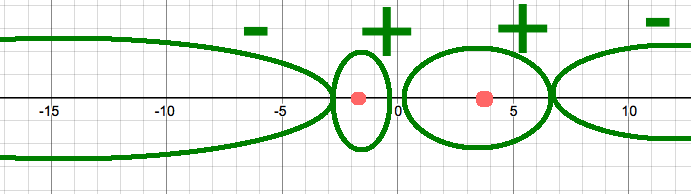
\includegraphics[width = 60mm]{images/722.png}
\end{center}
\noindent \textit{Розовым цветом на рисунке отмечены выколотые точки.} \\ \\

\noindent \textsl{3) Промежутки возрастания функции   $\Longleftrightarrow f'(x) > 0 $:}
\begin{gather*}
x = \begin{bmatrix}2(1 - \sqrt{7}), 0\end{bmatrix} \cup \begin{bmatrix}0, 2(1 + \sqrt{7})\end{bmatrix}
\end{gather*}

\noindent \textsl{4) Промежутки убывания функции   $\Longleftrightarrow f'(x) < 0 $:}
\begin{gather*}
x = \begin{bmatrix}-\infty, 2(1 - \sqrt{7})\end{bmatrix} \cup \begin{bmatrix}
2(1 + \sqrt{7}), \infty\end{bmatrix}
\end{gather*}

\noindent \textsl{5) Точки экстремума   $\Longleftrightarrow f'(x) = 0 $:}
\begin{align*}
 x &= 0 \\
 x &= 2(1 - \sqrt{7}) \\
 x &= 2(1 + \sqrt{7}) \\
\end{align*}

\noindent \textsl{6) Точки разрыва $ \Longleftrightarrow f'(x) $  - не определена:}
\begin{align*}
x &= -2 \\
x &= 4
\end{align*}

\noindent \textsl{7) Вторая производная:}
\begin{gather*}	
f''(x) = \frac{(-4x(x^2 - 4x - 24) - 2x^2(2x - 4))(x^2 - 2x + 8)^2 + 2x^2(x^2 - 4x - 24) \cdot 4(x - 1)(x^2 - 2x - 8) }{(x^2 - 2x + 8)^4} = \\
= \frac{-48x(x^2 + 4x + 16)}{(x^2 - 2x - 8)^3} = \frac{-48x(x^2 + 4x + 16)}{(x + 2)^3(x - 4)^3}
\end{gather*}

\begin{center}
	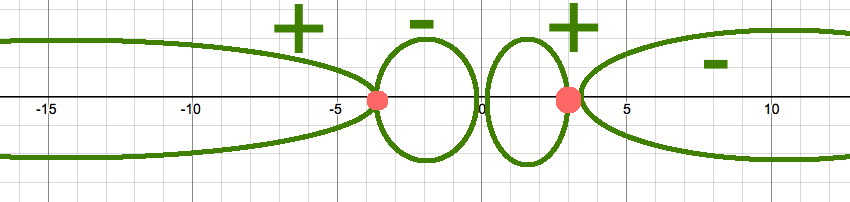
\includegraphics[width = 70mm]{images/723.png}
\end{center}
\noindent \textit{Розовым цветом на рисунке отмечены выколотые точки.} \\ \\
\noindent \textsl{8) Промежутки  выпуклости вниз $\Longleftrightarrow f''(x) > 0 $:}
\begin{gather*}
x = (-\infty, -2) \cup (0, 4)
\end{gather*}

\noindent \textsl{9) Промежутки  выпуклости вверх $\Longleftrightarrow f''(x) < 0 $:}
\begin{gather*}
 x = (-2, 0) \cup (4, \infty)
\end{gather*}
\noindent \textsl{10) Точки перегиба   $\Longleftrightarrow f''(x) = 0 $:}
\begin{align*}
x = 0 \quad y = 0
\end{align*}
\noindent \textsl{11) Ассимтоты:}
\begin{gather*}
k_1 = \lim_{x \to +\infty} \frac{f(x)}{x} = \frac{-2x^2}{x^2 - 2x - 8} = -2 \\
b_1 = \lim_{x \to +\infty} f(x) - kx = \frac{-2x^3}{x^2 - 2x - 8} + 2x = 
\frac{-2x^3 + 2x^3 - 4x^2 - 16x}{x^2 - 2x - 8} = \frac{- 4x^2 - 16x}{x^2 - 2x + 8} = -4 \\
\Rightarrow x \to -\infty: f(x) \to -2x - 4 \\ \\
k_2 = \lim_{x \to -\infty} \frac{f(x)}{x} = \frac{-2x^2}{x^2 - 2x - 8} = -2 \\
b_2 = \lim_{x \to +\infty} f(x) - kx = \frac{-2x^3}{x^2 - 2x - 8} + 2x = 
\frac{-2x^3 + 2x^3 - 4x^2 + 16x}{x^2 - 2x - 8} = \frac{- 4x^2 - 16x}{x^2 - 2x - 8} = -4 \\
\Rightarrow x \to -\infty: f(x) \to -2x - 4 
\end{gather*}
\newpage



%%%----------%%%----------%%%----------%%%----------%%%




3)
\begin{align*}
y = e^{\frac{1}{x^2 - 2x + 8}}
\end{align*} \\
\begin{center}
	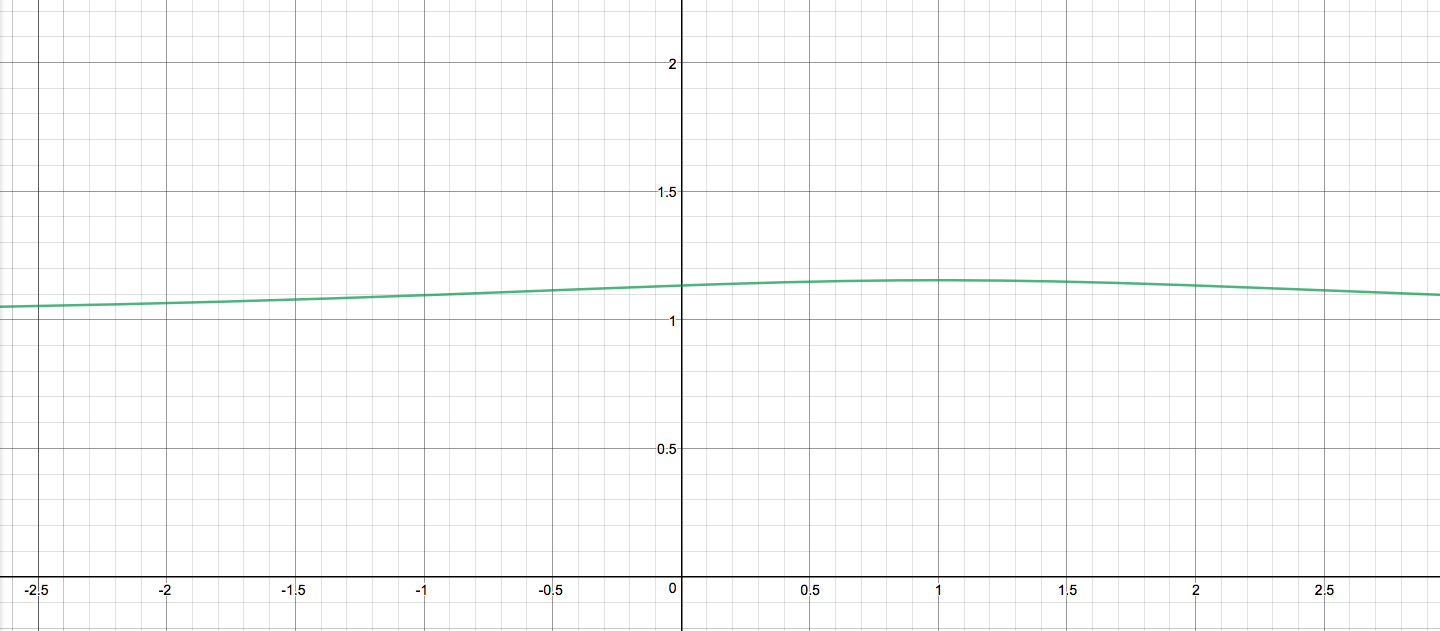
\includegraphics[width = 150mm]{images/731.png}
\end{center}

\noindent \textsl{1) ОДЗ:}
\begin{gather*}
x^2 - 2x + 8 \neq 0 \Rightarrow x - \textit{любое}
\end{gather*}

\noindent  \textsl{2) Первая производная:}
\begin{gather*}
f'(x) =  e^{\frac{1}{x^2 - 2x + 8}} \cdot \frac{-2(x - 1)}{(x^2 - 2x + 8)^2}
\end{gather*} 
\begin{center}
	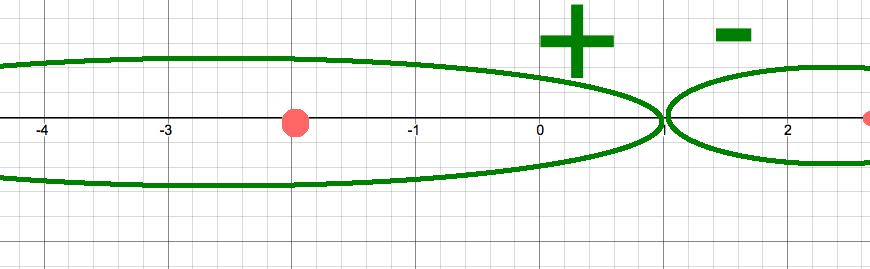
\includegraphics[width = 70mm]{images/732.png}
\end{center}

\noindent \textsl{3) Промежутки возрастания функции   $\Longleftrightarrow f'(x) > 0 $:}
\begin{gather*}
x = (-\infty, 1)
\end{gather*}

\noindent \textsl{4) Промежутки убывания функции   $\Longleftrightarrow f'(x) < 0 $:}
\begin{gather*}
x = (1, +\infty)
\end{gather*}

\noindent \textsl{5) Точки экстремума   $\Longleftrightarrow f'(x) = 0 $:}
\begin{align*}
x = 1
\end{align*}

\noindent \textsl{6) Точки разрыва $ \Longleftrightarrow f'(x) $  - не определена:}
\begin{align*}
\cdots
\end{align*}

\noindent \textsl{7) Вторая производная:}
\begin{gather*}	
f''(x) = (e^{\frac{1}{x^2 - 2x + 8}} \cdot \frac{-2(x - 1)}{(x^2 - 2x + 8)^2}) \cdot  \frac{-2(x - 1)}{(x^2 - 2x + 8)^2} + \\
+ e^{\frac{1}{x^2 - 2x + 8}}\cdot(-2)\cdot\frac{(x^2 - 2x + 8)^2 - (x - 1)(2(x^2 - 2x + 8)(2x - 2))}{(x^2 - 2x + 8)^4} = \\
= \frac{2e^{\frac{1}{x^2 - 2x + 8}}(3x^4 - 12x^3 + 34x^2 - 44x - 30)}{(x^2 - 2x + 8)^4}
\end{gather*}

\textit{\footnotesize Подобрать корни для многочлена 4 степени, стоящего в числителе, к сожалению, нам не удается, поэтому мы восопользуемся советом Лепского и будем использовать Wolphram Alpha } \\[4pt] \\
$ 3x^4 - 12x^3 + 34x^2 - 44x - 30 $ - \textit{имеет 2 вещесвенных корня: $ x_1 = -0,47488, \; x_2 = 2,4749 $}

\begin{center}
	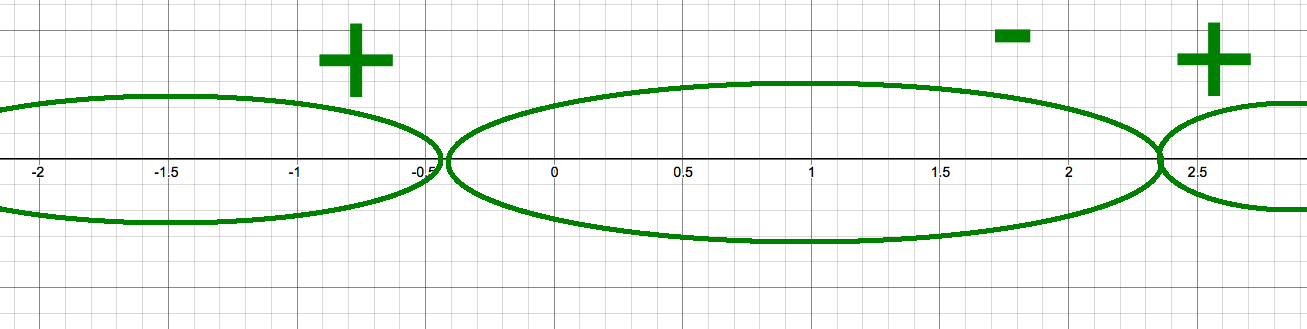
\includegraphics[width = 70mm]{images/733.png}
\end{center}
\noindent \textsl{8) Промежутки  выпуклости вниз $\Longleftrightarrow f''(x) > 0 $:}
\begin{gather*}
x = (-\infty, -0.47) \cup (2.47, \infty)
\end{gather*}

\noindent \textsl{9) Промежутки  выпуклости вверх $\Longleftrightarrow f''(x) < 0 $:}
\begin{gather*}
x = (-0.47, 2.47)
\end{gather*}

\noindent \textsl{10) Точки перегиба   $\Longleftrightarrow f''(x) = 0 $:}
\begin{align*}
x &= 0.47 \quad y = 1.15 \\[2pt]
x &= 2.47 \quad y = 1.12
\end{align*}
\noindent \textsl{11) Ассимтоты:}
\begin{gather*}
k_1 = \lim_{x \to +\infty} \frac{f(x)}{x} = \lim_{x \to +\infty} \frac{e^{\frac{1}{x^2 - 2x + 8}}}{x} = 0 \\
b_1 = \lim_{x \to +\infty} f(x) - kx = \lim_{x \to +\infty} e^{\frac{1}{x^2 - 2x + 8}} = 1 \\ 
\Rightarrow x \to +\infty: f(x) \to 1
\end{gather*}
\begin{gather*}
k_2 = \lim_{x \to -\infty} \frac{f(x)}{x} = \lim_{x \to -\infty} \frac{e^{\frac{1}{x^2 - 2x + 8}}}{x} = 0 \\
b_2 = \lim_{x \to -\infty} f(x) - kx = \lim_{x \to -\infty} e^{\frac{1}{x^2 - 2x + 8}} = 1 \\ 
\Rightarrow x \to -\infty: f(x) \to 1 \\ \\
\end{gather*}
\newpage





4)
\begin{align*}
y = e^{\frac{1}{x^2 - 2x - 8}}
\end{align*} \\
\begin{center}
	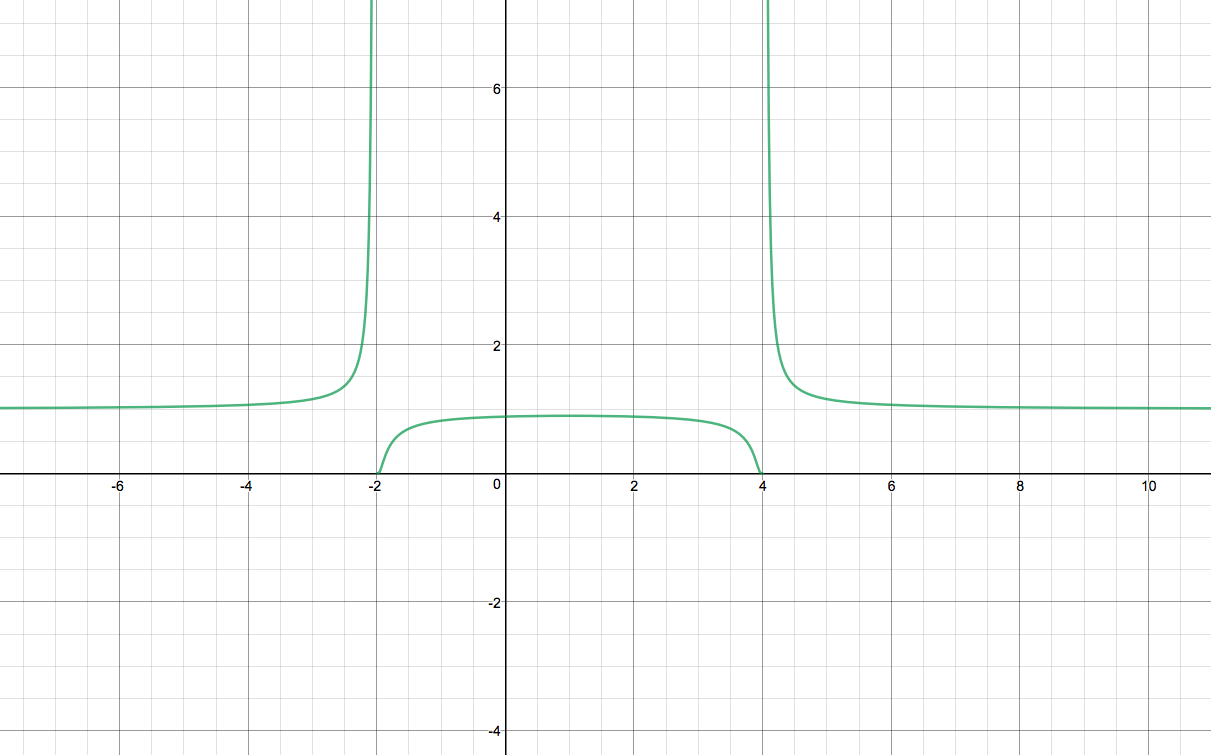
\includegraphics[width = 150mm]{images/741.png}
\end{center}

\noindent \textsl{1) ОДЗ:}
\begin{gather*}
x^2 - 2x - 8 \neq 0 \Rightarrow x \neq -2; 4
\end{gather*}

\noindent  \textsl{2) Первая производная:}
\begin{gather*}
f'(x) =  e^{\frac{1}{x^2 - 2x - 8}} \cdot \frac{-2(x - 1)}{(x^2 - 2x - 8)^2}
\end{gather*} 
\begin{center}
	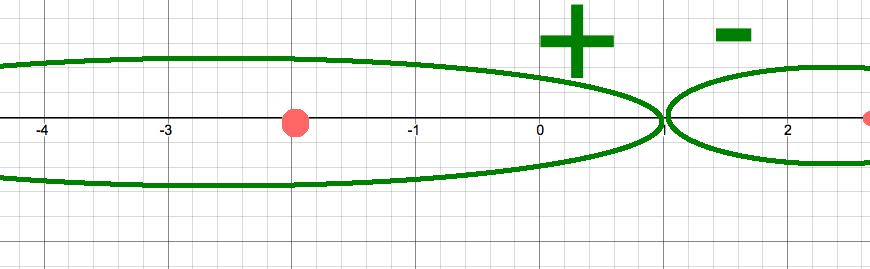
\includegraphics[width = 70mm]{images/732.png}
\end{center}
\noindent \textit{Розовым цветом на рисунке отмечены выколотые точки.} \\ \\

\noindent \textsl{3) Промежутки возрастания функции   $\Longleftrightarrow f'(x) > 0 $:}
\begin{gather*}
x = (-\infty, 1)
\end{gather*}

\noindent \textsl{4) Промежутки убывания функции   $\Longleftrightarrow f'(x) < 0 $:}
\begin{gather*}
x = (1, +\infty)
\end{gather*}

\noindent \textsl{5) Точки экстремума   $\Longleftrightarrow f'(x) = 0 $:}
\begin{align*}
x &= 1 \quad y = 0.89
\end{align*}

\noindent \textsl{6) Точки разрыва $ \Longleftrightarrow f'(x) $  - не определена:}
\begin{align*}
x &= -2 \\
x &= 4
\end{align*}

\noindent \textsl{7) Вторая производная:}
\begin{gather*}	
f''(x) =
(e^{\frac{1}{x^2 - 2x - 8}} \cdot \frac{-2(x - 1)}{(x^2 - 2x - 8)^2}) \cdot  \frac{-2(x - 1)}{(x^2 - 2x - 8)^2} + \\
+ e^{\frac{1}{x^2 - 2x - 8}}\cdot(-2)\cdot\frac{(x^2 - 2x - 8)^2 - (x - 1)(2(x^2 - 2x - 8)(2x - 2))}{(x^2 - 2x - 8)^4} = \\
= e^{\frac{1}{x^2 - 2x - 8}} \cdot \frac{2(3x^4 - 12x^3 + 2x^2 + 20x - 94)}{(x^2 - 2x - 8)^4}
\end{gather*}

\textit{\footnotesize Снова сталкиваемся с многочленом 4 степени и снова обращаемся к Wolphram Alpha} \\[4pt] \\
$ 3x^4 - 12x^3 + 2x^2 + 20x - 94 $ - \textit{имеет 2 вещественных корня: $ x_1 = -1.9167, \; x_2 = 3.9167 $}

\begin{center}
	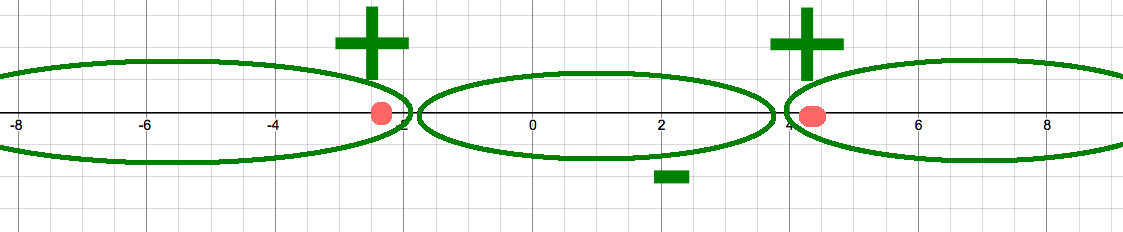
\includegraphics[width = 70mm]{images/743.png}
\end{center}
\noindent \textit{Розовым цветом на рисунке отмечены выколотые точки.} \\ \\
\noindent \textsl{8) Промежутки  выпуклости вниз $\Longleftrightarrow f''(x) > 0 $:}
\begin{gather*}
x = (-\infty, -1.91) \cup (3.92, \infty)
\end{gather*}

\noindent \textsl{9) Промежутки  выпуклости вверх $\Longleftrightarrow f''(x) < 0 $:}
\begin{gather*}
x = (-1.91, 3.92)
\end{gather*}

\noindent \textsl{10) Точки перегиба   $\Longleftrightarrow f''(x) = 0 $:}
\begin{align*}
&x = -1.91 \quad y = 0.15\\
&x = 3.92  \quad y = 0.12
\end{align*}
\noindent \textsl{11) Ассимтоты:}
\begin{gather*}
k_1 = \lim_{x \to +\infty} \frac{f(x)}{x} = \lim_{x \to +\infty} \frac{e^{\frac{1}{x^2 - 2x - 8}}}{x} = 0 \\
b_1 = \lim_{x \to +\infty} f(x) - kx = \lim_{x \to +\infty} e^{\frac{1}{x^2 - 2x - 8}} = 1 \\ 
\Rightarrow x \to +\infty: f(x) \to 1 \\ \\
k_2 = \lim_{x \to -\infty} \frac{f(x)}{x} = \lim_{x \to -\infty} \frac{e^{\frac{1}{x^2 - 2x - 8}}}{x} = 0 \\
b_2 = \lim_{x \to -\infty} f(x) - kx = \lim_{x \to -\infty} e^{\frac{1}{x^2 - 2x - 8}} = 1 \\ 
\Rightarrow x \to -\infty: f(x) \to 1 \\ \\
\end{gather*}
\newpage




%%%----------%%%----------%%%----------%%%----------%%%







\newpage
\textbf{\large Задача 8}
\medskip\hrule\medskip
\textsl{Исследуйте функцию с помощью производных первого и второго порядка, постройте эскиз ее графика(2):}
\begin{align*}
y = \ln \frac{x}{x + 2} + 1
\end{align*} \\

\begin{center}
	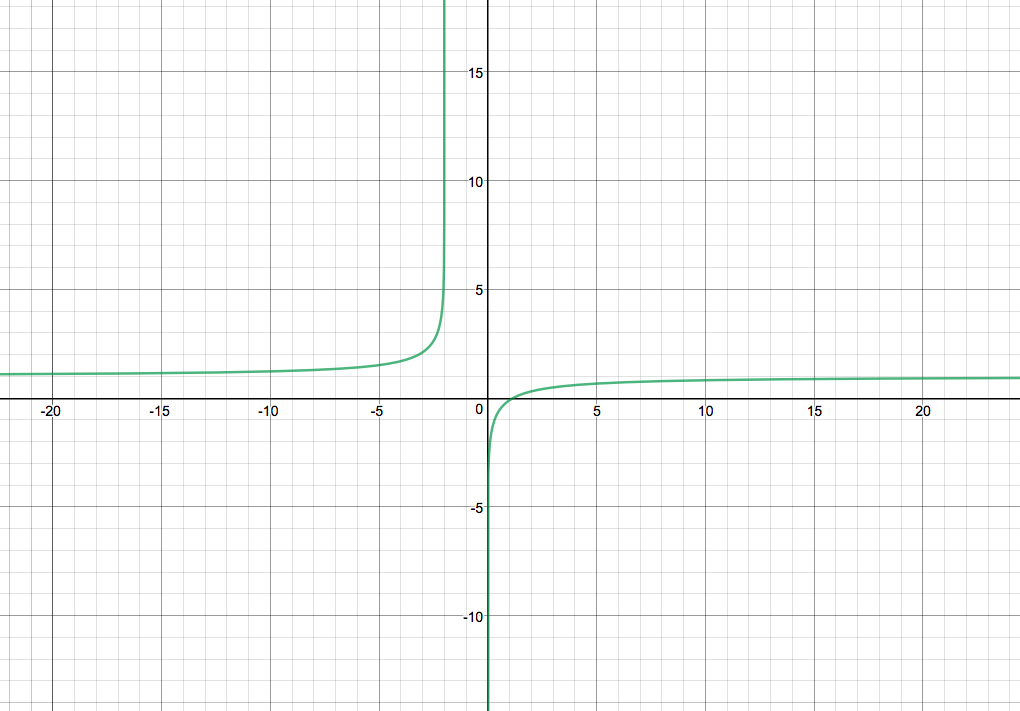
\includegraphics[width = 150mm]{images/81.png}
\end{center}

\noindent \textsl{1) ОДЗ:}
\begin{gather*}
	\frac{x}{x + 2} > 0 \Rightarrow x \subset (-\infty, 0) \cup (2, \infty)
\end{gather*}

\noindent \textsl{2) Первая производная:}
\begin{gather*}
f'(x) = \frac{1}{(\frac{x}{x + 2})} \cdot \frac{x + 2 - x}{(x + 2)^2} = \frac{2}{x(x + 2)}
\end{gather*} 
\begin{center}
	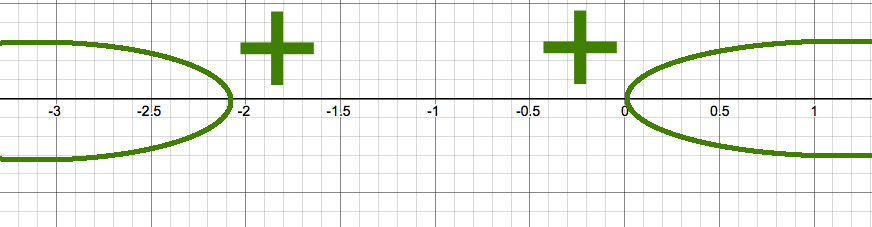
\includegraphics[width = 70mm]{images/82.png}
\end{center}

\noindent \textsl{3) Промежутки возрастания функции   $\Longleftrightarrow f'(x) > 0 $:}
\begin{gather*}
x = (-\infty, 0) \cup (2, \infty)
\end{gather*}

\noindent \textsl{4) Промежутки убывания функции   $\Longleftrightarrow f'(x) < 0 $:}
\begin{gather*}
\cdots
\end{gather*}

\noindent \textsl{5) Точки экстремума   $\Longleftrightarrow f'(x) = 0 $:}
\begin{align*}
\cdots
\end{align*}

\noindent \textsl{6) Точки разрыва $ \Longleftrightarrow f'(x) $  - не определена:}
\begin{align*}
	x &= 0 \quad f'(x) = +\infty \quad y \rightarrow +\infty\\
	x &= 2 \quad f'(x) = +\infty \quad y \rightarrow -\infty
\end{align*}

\noindent \textsl{7) Вторая производная:}
\begin{gather*}	
f''(x) = (f'(x))' = -\frac{2(2x + 2)}{(x(x + 2))^2} = -\frac{4(x + 1)}{(x(x + 2))^2}
\end{gather*}


\begin{center}
	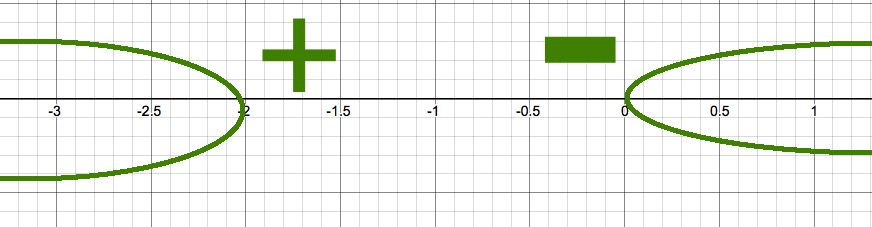
\includegraphics[width = 70mm]{images/83.png}
\end{center}
\noindent \textsl{8) Промежутки  выпуклости вниз $\Longleftrightarrow f''(x) > 0 $:}
\begin{gather*}
x = (-\infty, -2)
\end{gather*}

\noindent \textsl{9) Промежутки  выпуклости вверх $\Longleftrightarrow f''(x) < 0 $:}
\begin{gather*}
x = (0, +\infty)
\end{gather*}

\noindent \textsl{10) Точки перегиба   $\Longleftrightarrow f''(x) = 0 $:}
\begin{align*}
 \cdots
\end{align*}

\noindent \textsl{11) Ассимтоты:}
\begin{gather*}
k_1 = \lim_{x \to +\infty} \frac{f(x)}{x} = \lim_{x \to +\infty} \frac{\ln \frac{x}{x + 2}}{x} + \frac{1}{x} = 0 \\
b_1 = \lim_{x \to +\infty} f(x) - kx = \lim_{x \to +\infty} \ln \frac{x}{x + 2} + 1 = 1 \\
\Rightarrow x \to +\infty: f(x) \to 1 \\ \\
k_2 = \lim_{x \to -\infty} \frac{f(x)}{x} = \lim_{x \to -\infty} \frac{\ln \frac{x}{x + 2}}{x} + \frac{1}{x} = 0 \\
b_2 = \lim_{x \to -\infty} f(x) - kx = \lim_{x \to +\infty} \ln \frac{x}{x + 2} + 1 = 1 \\
\end{gather*}
\newpage







%%%----------%%%----------%%%----------%%%----------%%%










\textbf{\large Задача 9}
\medskip\hrule\medskip
\textsl{Исследуйте функцию с помощью производных первого и второго порядка, постройте эскиз ее графика(6):}
\begin{align*}
y = \frac{x^2 + 2x + 2}{x^2 + 3x + 2}
\end{align*} \\

\begin{center}
	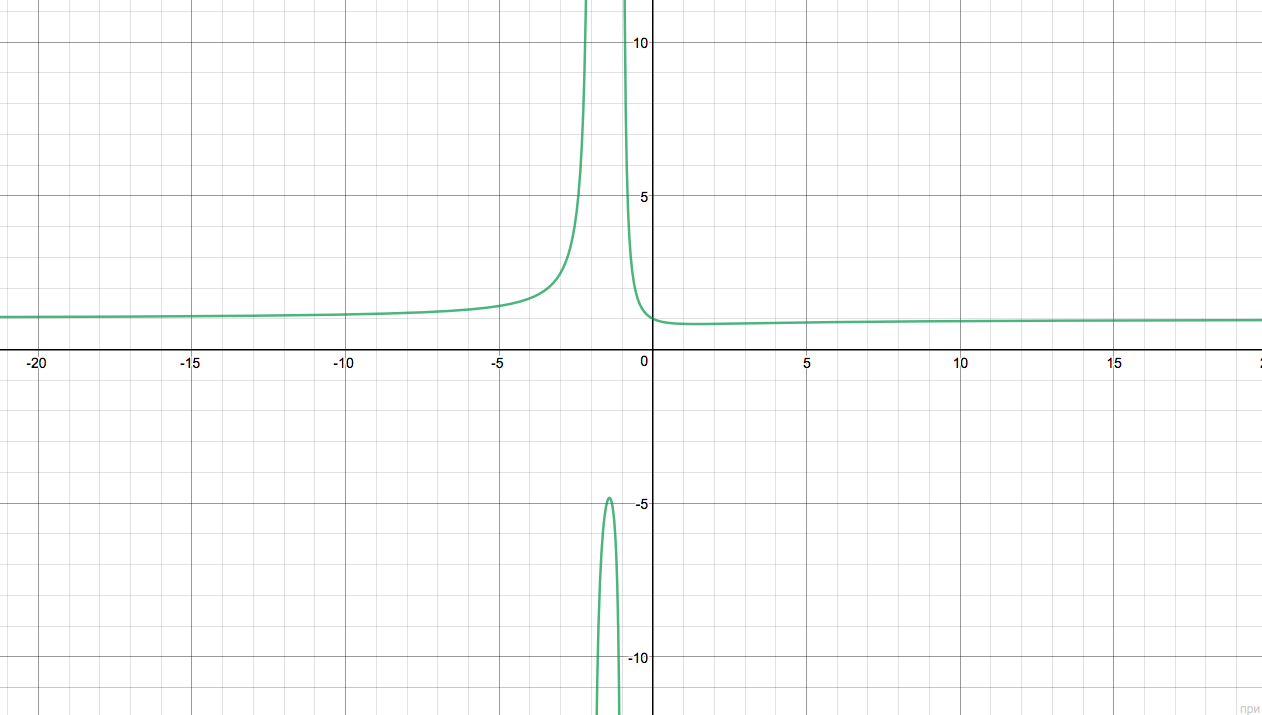
\includegraphics[width = 150mm]{images/91.png}
\end{center}

\begin{gather*}
	y = \frac{x^2 + 2x + 2}{x^2 + 3x + 2} = \frac{x^2 + 3x + 2 - x}{x^2 + 3x + 2} = 1 - \frac{x}{x^2 + 3x + 2}
\end{gather*}

\noindent \textsl{1) ОДЗ:}
\begin{gather*}
x^2 + 3x + 2 \neq 0 \Rightarrow x \neq -1, -2
\end{gather*}

\noindent  \textsl{2) Первая производная:}
\begin{gather*}
f'(x) = -\frac{(x^2 + 3x + 2) - x(2x + 3)}{(x^2 + 3x + 2)^2} = \frac{x^2 - 2}{(x^2 + 3x + 2)^2}
\end{gather*} 
\begin{center}
	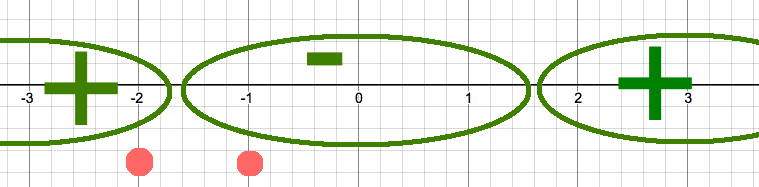
\includegraphics[width = 70mm]{images/92.png}
\end{center}

\noindent \textit{Розовым цветом на рисунке отмечены выколотые точки.} \\ \\
\noindent \textsl{3) Промежутки возрастания функции   $\Longleftrightarrow f'(x) > 0 $:}
\begin{gather*}
x = (-\infty, -\sqrt{2}) \cup (\sqrt{2}, +\infty)
\end{gather*}

\noindent \textsl{4) Промежутки убывания функции   $\Longleftrightarrow f'(x) < 0 $:}
\begin{gather*}
x = (-\sqrt{2}, \sqrt{2})
\end{gather*}

\noindent \textsl{5) Точки экстремума   $\Longleftrightarrow f'(x) = 0 $:}
\begin{align*}
&x = \sqrt{2} \quad y = 0.83 \\
&x = -\sqrt{2} \quad y = -4.82
\end{align*}

\noindent \textsl{6) Точки разрыва $ \Longleftrightarrow f'(x) $  - не определена:}
\begin{align*}
x &= -2-0 \quad f'(x) = +\infty \quad y \rightarrow +\infty\\
x &= -2+0 \quad f'(x) = +\infty \quad y \rightarrow -\infty\\
x &= -1-0 \quad f'(x) = -\infty \quad y \rightarrow -\infty \\
x &= -1+0 \quad f'(x) = -\infty \quad y \rightarrow +\infty \\
\end{align*}

\noindent \textsl{7) Вторая производная:}
\begin{gather*}	
f''(x) = (f'(x))' = \frac{2x(x^2 + 3x + 2)^2 - (x^2 - 2)2(x^2 + 3x + 2)(2x + 3)}{(x^2 + 3x + 2)^4} = \\
= \frac{2x^3 + 6x^2 + 4x - 4x^3 - 6x^2 + 8x + 12}{(x^2 + 3x + 2)^3} = \frac{-2x^3 + 12x + 12}{(x^2 + 3x + 2)^3} = \frac{2(-x^3 + 6x + 6)}{(x^2 + 3x + 2)^3} = \\
= \frac{2x^3 + 6x^2 + 4x - 4x^3 - 6x^2 + 8x + 12}{(x^2 + 3x + 2)^3} = \frac{-2x^3 + 12x + 12}{(x^2 + 3x + 2)^3} = \frac{-2(x^3 - 6x - 6)}{(x + 1)^3(x + 2)^3} = \\
= \frac{2}{(x + 1)^3} - \frac{4}{(x + 2)^3}\\
\end{gather*}

\textit{\footnotesize И снова корни многочлена очень трудно подобрать самому, поэтому мы идем к Wolphram Alpha :)} \\[4pt] \\
$ x^3 - 6x - 6 $ \textit{ - имеет один корень $ x_0 = \sqrt[3]{2} + 2^{2/3} \approx 2,8473$} \\
\begin{center}
	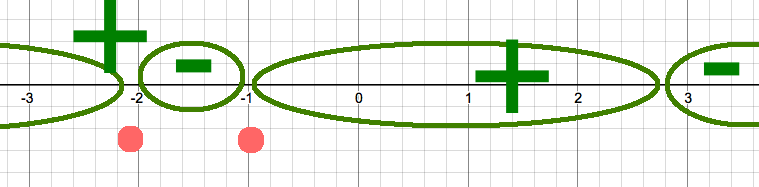
\includegraphics[width = 70mm]{images/93.png}
\end{center}
\noindent \textsl{8) Промежутки  выпуклости вниз $\Longleftrightarrow f''(x) > 0 $:}
\begin{gather*}
x = (-\infty, -2) \cup (-1, \; 2.85)
\end{gather*}

\noindent \textsl{9) Промежутки  выпуклости вверх $\Longleftrightarrow f''(x) < 0 $:}
\begin{gather*}
x = (-2, -1) \cup (2.85 \; , +\infty) 
\end{gather*}

\noindent \textsl{10) Точки перегиба   $\Longleftrightarrow f''(x) = 0 $:}
\begin{align*}
x = 2.85 \quad y = 2.85
\end{align*}
\noindent \textsl{11) Ассимтоты:}
\begin{gather*}
	k_1 = \lim_{x \to +\infty} \frac{f(x)}{x} = \lim_{x \to +\infty} \frac{x + 2 + \frac{2}{x}}{x^2 + 3x + 2} = 0 \\
	b_1 = \lim_{x \to +\infty} f(x) - kx = \frac{x^2 + 2x + 2}{x^2 + 3x + 2} = 1 \\
	\Rightarrow x \to +\infty: f(x) \to 1 \\ \\
	k_2 = \lim_{x \to -\infty} \frac{f(x)}{x} = \lim_{x \to -\infty} \frac{x + 2 + \frac{2}{x}}{x^2 + 3x + 2} = 0 \\
	b_2 = \lim_{x \to -\infty} f(x) - kx = \frac{x^2 + 2x + 2}{x^2 + 3x + 2} = 1 \\
	\Rightarrow x \to -\infty: f(x) \to 1 \\
\end{gather*}
\newpage



%%%----------%%%----------%%%----------%%%----------%%%





\textbf{\large Задача 10}
\medskip\hrule\medskip
\textsl{Исследуйте и постройте эскизы кривых (в б перейдите к полярным координатам) (10)}
\begin{equation}
\textsl{a) }
	\begin{cases}
		x(t) = \frac{1}{3}t^3 + \frac{7}{2}t^2 - 8t \\ 
		y(t) = \frac{1}{3}t^3 + t^2 - 48t \\ 
	\end{cases}
	\\
\textsl{б) } 
	x^4 + y^4 = x^2y^2
\end{equation}
a)
\begin{center}
	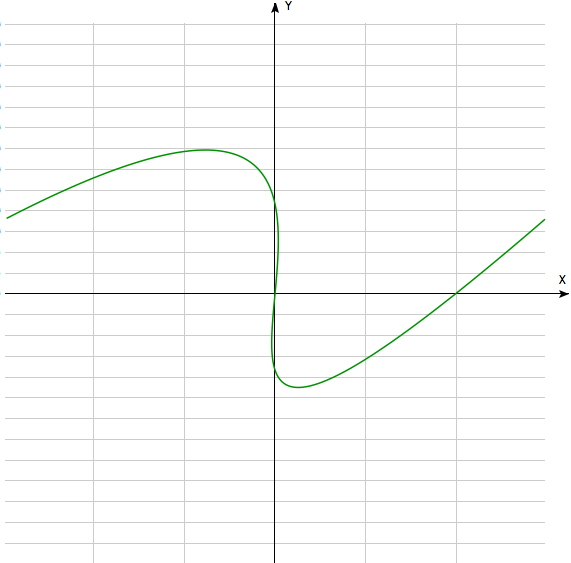
\includegraphics[width = 50mm]{images/101.png}
\end{center}

\noindent \textsl{1) ОДЗ:}
\begin{gather*}
\cdots
\end{gather*}

\noindent  \textsl{2) Первая производная:}
\begin{gather*}
y'_t = (\frac{1}{3}t^3 + t^2 - 48t)' = t^2 + 2t - 48 \\
x'_t = (\frac{1}{3}t^3 + \frac{7}{2}t^2 - 8t)' = t^2 + 7t - 8 \\
y'_x = \frac{t^2 + 2t - 48}{t^2 + 7t - 8} = \frac{t - 6}{t - 1}
\end{gather*} 

\noindent \textsl{3) Промежутки возрастания функции   $\Longleftrightarrow f'(x) > 0 $:}
\begin{gather*}
t = (-\infty, 1) \cup (6, +\infty)
\end{gather*}

\noindent \textsl{4) Промежутки убывания функции   $\Longleftrightarrow f'(x) < 0 $:}
\begin{gather*}
t = (1, 6)
\end{gather*}

\noindent \textsl{5) Точки экстремума   $\Longleftrightarrow f'(x) = 0 $:}
\begin{align*}
t = 6
\end{align*}

\noindent \textsl{6) Точки разрыва $ \Longleftrightarrow f'(x) $  - не определена:}
\begin{align*}
t &= 8
\end{align*}

\noindent \textsl{7) Вторая производная:}
\begin{gather*}	
y''_t = (y'_t)' = 2(t + 1) \\
y''_x = \dfrac{2(t + 1)}{(t - 1)(t + 8)}
\end{gather*}

\noindent \textsl{8) Промежутки  выпуклости вниз $\Longleftrightarrow f''(x) > 0 $:}
\begin{gather*}
t = (-8, -1) \cup (1, +\infty)
\end{gather*}

\noindent \textsl{9) Промежутки  выпуклости вверх $\Longleftrightarrow f''(x) < 0 $:}
\begin{gather*}
t = (-\infty , -8) \cup (-1, 1) 
\end{gather*}

\noindent \textsl{10) Точки перегиба   $\Longleftrightarrow f''(x) = 0 $:}
\begin{align*}
t = -1
\end{align*}
\noindent \textsl{11) Ассимтоты:}
\begin{gather*}
k_1 = \lim_{x \to +\infty} \frac{f(x)}{x} = \lim_{x \to +\infty} \frac{\frac{1}{3}t^3 + t^2 - 48t}{\frac{1}{3}t^3 + \frac{7}{2}t^2 - 8t} = 1 \\
b_1 = \lim_{x \to +\infty} f(x) - kx = \frac{-\frac52x^2 - 40t}{\frac{1}{3}t^3 + \frac{7}{2}t^2 - 8t} = 0 \\
\Rightarrow x \to +\infty: f(x) \to x \\ \\
k_2 = \lim_{x \to -\infty} \frac{f(x)}{x} = \lim_{x \to -\infty} \frac{\frac{1}{3}t^3 + t^2 - 48t}{\frac{1}{3}t^3 + \frac{7}{2}t^2 - 8t} = 1 \\
b_2 = \frac{-\frac52x^2 - 40t}{\frac{1}{3}t^3 + \frac{7}{2}t^2 - 8t} = 0 \\
\Rightarrow x \to -\infty: f(x) \to x \\
\end{gather*}
\\ \\ \\
б)

\begin{gather*}
x^4 + y^4 = x^2y^2 \\[2pt]
y = \rho \sin t \quad x = \rho \cos t \\[2pt]
\rho^4(\sin^4 t + \cos^4 t - \sin^2t \cos^2t) = 0
\end{gather*}
Отметим,что в тех случаях, когда $ \sin^4 t + \cos^4 t - \sin^2t \cos^2t \neq 0 $, $ \rho(t)  $ получается равным 0, поэтому наш график выраждается в точку. Если же наоборот, выражение равно 0, это значит, что на графике мы имеем луч из 0.
\begin{gather*}
\sin^4 t + \cos^4 t - \sin^2t \cos^2t = 0 \\[2pt]
1)\cos 4t = \cos (2t + 2t) = \cos^2 2t - \sin^2 2t = (2\cos^2t - 1)^2 - (2\sin t \cos t)^2 =\\[2pt]
= 4\cos^4t - 4\cos^2t + 1 - 4\sin^2 t \cos^2 t =
4\cos^4t - 4\cos^2t(1 + \sin^2 t) + 1 = \\[2pt]
4\cos^4t - 4(1 - \sin^2 t)(1 + \sin^2 t) + 1 = 4\cos^4t + 4\sin^4t - 3\\[2pt]
2)\sin^2t \cos^2t = (\sin t \cos t)^2 = \frac14 (\sin2t)^2 = \frac18(1 - \cos(4t))
\end{gather*}
Теперь собираем все вместе
\begin{gather*}
\sin^4 t + \cos^4 t - \sin^2t \cos^2t = \frac14(\cos4t + 3) - \frac18(1 - \cos(4t) = \frac18 (3\cos4t + 5) = 0 \Rightarrow \cos4t = -\frac53 \Rightarrow\\[2pt] 
\Rightarrow \text{не выполняется не при каких }t \Rightarrow \text{график есть просто точка}
\end{gather*}

%%%----------%%%----------%%%----------%%%----------%%%






\newpage
\textbf{\large Задача 11}
\medskip\hrule\medskip
\textsl{Найдите интегралы(14):}
\begin{align*}
	\int \frac{2^x \sqrt{\arctan \big (\dfrac{2^x}5 \big )}}{25 + 4^x}dx
\end{align*} \\

Сделаем первую замену $ v = 2^x \Rightarrow dv = d(e^{\ln2 \cdot x}) = e^{\ln2x} \cdot ln2 \cdot dx = 2^x \cdot ln2 \cdot dx$
\begin{gather*}
	 \int \frac{\sqrt{\arctan(\frac{v}{5})}}{(25 + v^2) \cdot ln2}dv
\end{gather*}
После этого нам понадобиться еще одна замена: $ u = \arctan(\frac{v}5) $ \\
$ \Rightarrow du = \dfrac{(\frac{dv}{5})}{1 + \frac{v^2}{25}} = 5 \cdot \dfrac{dv}{25 + v^2} $
\begin{gather*}
	\int \frac{\sqrt{u}du}{5 \cdot ln2} = \frac{2u^{\frac{3}{2}}}{15 \cdot ln2} + C = \frac{2(\arctan(\frac{v}{5}))^{\frac{3}{2}}}{15 \cdot ln2} + C = 
	\frac{2(\arctan(\frac{2^x}{5}))^{\frac{3}{2}}}{15 \cdot ln2} + C
\end{gather*}
\\ \\ \\



%%%----------%%%----------%%%----------%%%----------%%%




\textbf{\large Задача 12}
\medskip\hrule\medskip
\textsl{Найдите интегралы(18):}
\begin{align*}
\textsl{а) } \int \frac{dx}{x - 10\sqrt[9]{x^5}}, \quad \textsl{б) }  \int \frac{dx}{x\sqrt{9 - x^2}}
\end{align*} \\

\textsl{a) } Сделаем первую замену: $ v = \sqrt[9]{x} \Rightarrow dv = \frac{dx}{9\sqrt[9]{x^8}} \Rightarrow dx = 9v^8 dv$
\begin{gather*}
	\int \frac{dx}{x - 10\sqrt[9]{x^5}} = \int \frac{9v^8dv}{v^5(v^4 - 10)} = \int \frac{9v^3dv}{v^4 - 10}
\end{gather*}
После этого нам понадобиться еще одна замена: $ u = v^4 - 10 \Rightarrow du = 4v^3dv $
\begin{gather*}
	\int \frac{9du}{4u} = \frac{9}{4} \ln |u| + C = \frac{9}{4} \ln |v^4 - 10| + C = \frac{9}{4} \ln |\sqrt[9]{x^4} - 10| + C 		
\end{gather*}
\\
\textsl{б) } Сделаем первую замену: $ v = \sqrt{9 - x^2} \Rightarrow dv = \frac{-xdx}{\sqrt{9 - x^2}}$
\begin{gather*}
	\int \frac{dx}{x\sqrt{9 - x^2}} = \int \frac{-dv}{x^2} = \int \frac{-dv}{9 - v^2} = \int \frac{dv}{v^2 - 3^2} = \frac{1}{6}\ln \bigg|\frac{v - 3}{v + 3} \bigg|	+ C = \frac{1}{6}\ln \bigg|\frac{\sqrt{9 - x^2} - 3}{\sqrt{9 - x^2} + 3} \bigg|	+ C
\end{gather*} 
\newpage




%%%----------%%%----------%%%----------%%%----------%%%



\textbf{\large Задача 13}
\medskip\hrule\medskip
\textsl{Найдите интегралы(22):}
\begin{align*}
	\textsl{a) } 
	\int xe^{3x}dx \qquad
	\textsl{б) }
	\int (x^2 - 5x + 3) \cos (2x) \; dx \qquad
	\textsl{в) }
	\int e^{-4x} \sin (3x) \; dx
\end{align*} \\ 

Мы будем интегрировать по частям \\[2pt]
\textsl{a) } 
\begin{gather*}
	\int xe^{3x}dx = \int x d(\frac{e^{3x}}{3}) = \frac{xe^{3x}}{3} - \int \frac{e^{3x}dx}{3} + C = 
	\frac{xe^{3x}}{3} - \frac{e^{3x}}{9} + C = \frac{(3x - 1)e^{3x}}{9} + C
\end{gather*}

\noindent \textsl{б) }
\begin{gather*}
	\int (x^2 - 5x + 3) \cos (2x) \;dx = \int (x^2 - 5x + 3) d(\frac{\sin 2x}2) = 
	\frac{(x^2 - 5x + 3)  \sin (2x)}2 - \int \frac{(2x - 5)\sin (2x) dx}{2} + \\[2pt] +  \; C = 
	\frac{(x^2 - 5x + 3)  \sin (2x)}2 - \int \frac{(2x - 5)d(-\cos(2x)))}{4} + C = 
	\frac{(x^2 - 5x + 3)  \sin (2x)}2 + \frac{(2x - 5)\cos(2x)}{4} + \\[2pt] + \int \frac{-\cos(2x)dx}{2} + C = 
	\frac{(x^2 - 5x + 3)  \sin (2x)}2 + \frac{(2x - 5)\cos(2x)}{4} -  \frac{\sin(2x)}{4} + C = \\[2pt] = \frac{(2x^2 - 10x + 5)\sin (2x) + (2x - 5)\cos(2x)}{4}
\end{gather*}
\noindent \textsl{в) } 
\begin{gather*}
	\int e^{-4x} \sin (3x) \; dx = \int e^{-4x} d(\frac{-\cos (3x)}{3}) = \frac{-e^{-4x} \cos 3x}{3} - \int (-4)e^{-4x} \frac{-\cos (3x)}{3}dx + C = \\[2pt]
	= \frac{-e^{-4x} \cos (3x)}{3} + \int 4e^{-4x} d(\frac{-\sin (3x)}{9}) + C = 
	\frac{-e^{-4x} \cos (3x)}{3} + \frac{-4e^{-4x} \sin (3x)}{9} - \\[2pt]
	- \int (-16)e^{-4x} \frac{-\sin (3x)}{9}dx + C  
	= \frac{-e^{-4x} \cos (3x)}{3} + \frac{-4e^{-4x} \sin (3x)}{9} - 
	\int \frac{16e^{-4x} \sin (3x)}{9}dx + C \Rightarrow	\\[2pt]
	(1 + \frac{16}9) \int e^{-4x} \sin (3x) dx = \frac{-e^{-4x} \cos (3x)}{3} - \frac{4e^{-4x} \sin (3x)}{9} + C \Rightarrow \\[2pt]
	\int e^{-4x} \sin (3x) dx = -\frac{3e^{-4x} \cos (3x)}{25} - \frac{4e^{-4x} \sin (3x)}{25} + C = -\frac{(4\sin(3x) + 3\cos(3x))e^{-4x}}{25} + C
\end{gather*}
\newpage



%%%----------%%%----------%%%----------%%%----------%%%






\textbf{\large Задача 14}
\medskip\hrule\medskip
\textsl{Найдите интегралы(26):}
\begin{align*}
	\textsl{a) } \int \frac{2x - 13}{x^2 + 2x + 37}dx \qquad
	\textsl{б) } \int \frac{5x + 9}{x^2 + 5x + 4}dx
\end{align*} \\ 

\textsl{a) } 
\begin{gather*}
	\int \frac{2x - 13}{x^2 + 2x + 37}dx = \int \frac{2x + 2 - 15}{x^2 + 2x + 37}dx = \int \frac{d(x^2 + 2x + 37) - 15dx}{x^2 + 2x + 37} = 
	\ln |x^2 + 2x + 37| - \\[2pt]
	 - \int \frac{15dx}{(x + 1)^2 + 36} + C = \ln |x^2 + 2x + 37| - \int \frac{15d(x + 1)}{36((\frac{x + 1}6)^2 + 1)} + C =  \ln |x^2 + 2x + 37| - \\[2pt]
	 - \frac{15}{6}\arctan(\frac{x + 1}6) + C = \ln |x^2 + 2x + 37| -  \frac{5}{2}\arctan(\frac{x + 1}6) + C
\end{gather*}

\textsl{б) }
\begin{gather*}
	\int \frac{5x + 9}{x^2 + 5x + 4}dx = \int \frac{\frac52(2x + 5) - \frac72}{x^2 + 5x + 4}dx = \int \frac{\frac52d(x^2 + 5x + 4) - \frac72dx}{x^2 + 5x + 4} = \\[2pt]
	= \frac52 \ln |x^2 + 5x + 4| - \frac72 \int \frac{d(x + \frac52)}{(x + \frac52)^2 - (\frac32)^2} = 
	\frac52 \ln |x^2 + 5x + 4| + \\[2pt]
	+ \frac72 \int \frac{d(x + \frac52)}{(\frac32)^2 - (x + \frac52)^2 } + C = 
	\frac52 \ln |x^2 + 5x + 4| + \\[2pt]
	+ \frac76 \ln \big |\frac{\frac32 + x + \frac52}{\frac32 - x - \frac52} \big | + C =
	\frac52 \ln |x^2 + 5x + 4| + \frac76 \ln \big |\frac{x + 4}{x + 1}\big | + C =  \\[2pt]
	\frac52 \ln |x + 1| + \frac52 |x + 4| + \frac76 \ln |x + 4| - \frac 76 \ln|x + 1| + C = \\[2pt] = \frac{11|x + 4| + 4|x + 1|}{3} + C	
\end{gather*}
\newpage


%%%----------%%%----------%%%----------%%%----------%%%


\textbf{\large Задача 15}
\medskip\hrule\medskip
\textsl{Найдите интегралы(30):}
\begin{align*}
	\textsl{a) } \int \frac{(4x + 3)dx}{(x + 3)^2(x^2 + x + 4)} \qquad
	\textsl{б) } \int \frac{(x^2 + x - 7)dx}{x^4 - 3x^3 - 8x + 24} \qquad
	\textsl{в) } \int \frac{(x^4 - 4x^3 + 2x^2 - 7)dx}{x^3 - 6x^2 + 5x}
\end{align*} \\

Воспользуемся методом неопределенных коэффицентов \\[2pt]

\textsl{а) }
\begin{gather*}
	\int \frac{(4x + 3)dx}{(x + 3)^2(x^2 + x + 4)} = \int \frac{Ax + B}{(x + 3)^2}dx + \int \frac{Cx + D}{x^2 + x + 4}dx \Rightarrow \\[2pt]
	4x + 3 = Ax^3 + Ax^2 + 4Ax + Bx^2 + Bx + 4B + Cx^3 + 6Cx^2 + 9Cx + Dx^2 + 6Dx + 9D = \\[2pt]
	= (A + C)x^3 + (A + B + 6C + D)x^2 + (4A + B + 9C + 6D)x + (4B + 9D) \Rightarrow
\end{gather*}
\begin{gather*}
\begin{cases}
A + C = 0 \\
A + B + 6C + D = 0 \\
4A + B + 9C + 6D = 4 \\
4B + 9D = 3	
\end{cases}
\begin{cases}
A + C = 0 \\
B + 5C + D = 0 \\
B + 5C + 6D = 4 \\
4B + 9D = 3	
\end{cases}
\begin{cases}
A = -C \\
D = \frac45 \\
B + 5C + \frac45 = 0\\
4B + \frac{36}5 = 3	
\end{cases}
\begin{cases}
A = -C = -\frac1{20}\\
D = \frac45 \\
C = \frac1{20} \\
B = -\frac{21}{20}
\end{cases}
\end{gather*}

\begin{gather*}
	\Rightarrow \int -\frac{(x + 21 )dx}{20(x + 3)^2} + \int \frac{(x + 16)dx}{20(x^2 + x + 4)} = 
	- \int \frac{d((x + 3)^2)}{40(x + 3)^2} - \int \frac{36d(x + 3)}{40(x + 3)^2} + \int \frac{d(x^2 + x + 4)}{40(x^2 + x + 4)} + \\[2pt] +  \int \frac{31d(x + \frac12)}{40((x + \frac12)^2 + \frac{15}4)} = - \frac{\ln (x + 3)^2}{40} + \frac{9}{10(x + 3)} + \frac{\ln |x^2 + x + 4|}{40} + \frac{31\sqrt{15}}{300}\arctan(\frac{2\sqrt{15}(x + \frac12)}{15}) + C =\\[2pt] = \frac{|x^2 + x + 4| - 2\ln|x + 3|}{40} + \frac{31\arctan(\frac{2x + 1}{\sqrt{15}})}{20\sqrt{15}} + \frac9{10(x + 3)} + C
\end{gather*}

\noindent \textsl{б) }
\begin{gather*}
	\int \frac{(x^2 + x - 7)dx}{x^4 - 3x^3 - 8x + 24} = \int \frac{(x^2 + x - 7)dx}{(x - 2)(x - 3)(x^2 + 2x + 4)} = \int \frac{A}{x - 2}dx + \int \frac{B}{x - 3}dx + \int \frac{Cx + D}{x^2 + 2x + 4}dx \\[2pt]
	x^2 + x - 7 =  (Ax - 3A)(x^2 + 2x + 4) + (Bx - 2B)(x^2 + 2x + 4) + (Cx + D)(x - 2)(x - 3) = \\[2pt]
	= Ax^3 - Ax^2 - 2Ax - 12A + Bx^3 - 8B + Cx^3 - 5Cx^2 + Dx^2 + 6Cx - 5Dx + 6D = \\[2pt]
	= (A + B + C)x^3 + (-A - 5C + D)x^2 + (-2A + 6C - 5D)x + (-12A - 8B + 6D) \Rightarrow
\end{gather*}

\begin{gather*}
\begin{cases}
A + B + C = 0 \\
- A - 5C + D = 1 \\
-2A + 6C - 5D = 1 \\
-12A - 8B + 6D = -7
\end{cases}
\begin{cases}
A + B + C = 0 \\
B - 4C + D = 1 \\
2B + 8C - 5D = 1 \\
4B + 12C + 6D = -7 \\
\end{cases}
\begin{cases}
A + B + C = 0 \\
B - 4C + D = 1 \\
16C - 7D = -1 \\
28C +2D = -11 \\
\end{cases}
\begin{cases}
A + B + C = 0 \\
B - 4C + D = 1 \\
57D = -37 \\
-4C +16D = -9 \\
\end{cases}
\end{gather*} \\
$ A =  \frac1{12} \quad B =  \frac{5}{19} \quad C =  -\frac{79}{228} \quad D = -\frac{37}{57} $

\begin{gather*}
	\int \frac{d(x - 2)}{12(x - 2)} + \int \frac{5d(x - 3)}{19(x - 3)} + \int \frac{-\frac{79}{456}d(x^2 + 2x + 4 )}{x^2 + 2x + 4 } - \int \frac{23}{76((x + 1)^2 + 3)} = \\[2pt]
	= \frac{\ln |x - 2|}{12} + \frac{5\ln |x - 3|}{19} - \frac{79\ln |x^2 + 2x + 4|}{456} - \frac{23}{76\sqrt{3}} \arctan (\frac{x + 1}{\sqrt{3}}) + C
\end{gather*}



\noindent \textsl{в) }
\begin{gather*}
	\int \frac{(x^4 - 4x^3 + 2x^2 - 7)dx}{x^3 - 6x^2 + 5x} = 
	\int (x + 2)dx + \int \frac{9x^2 - 10x - 7}{x(x - 5)(x - 1)}dx = \\[2pt]
	= \int (x + 2)dx + \int \frac{Adx}{x} + \int \frac{Bdx}{x - 1} + \int \frac{Cdx}{x - 5} \Rightarrow  9x^2 - 10x - 7 = A(x - 1)(x - 5) \; + \\[2pt] + \; Bx(x - 5) + Cx(x - 1)
	= (A + B + C)x^2 - (6A + 5B + C)x + 5A
\end{gather*}
\begin{gather*}
\begin{cases}
A + B + C = 9 \\
6A + 5B + C = 10 \\
5A = -7
\end{cases}
\begin{cases}
B + C = \frac{52}5 \\
5B + C = \frac{92}5 \\
A = -\frac75
\end{cases}
\begin{cases}
A = -\frac75 \\
B = 2 \\
C = \frac{42}5 \\
\end{cases}
\end{gather*}

\begin{gather*}
	\int (x + 2)dx - \int \frac{7dx}{5x}  + \int \frac{2d(x - 1)}{x - 1} + \int \frac{42d(x - 5)}{5(x - 5)} = \\
	= \frac{(x + 2)^2}{2} - \frac{7\ln|x|}{5}  + 2\ln|x - 1| +  \frac{42\ln |x - 5|}{5} + C
\end{gather*}
\\ \\ \\


\textbf{\large Задача 16}
\medskip\hrule\medskip
\textsl{Найдите интегралы(4):}
\begin{align*}
	\textsl{a) } \int \sin^2x \cos^4x \; dx \qquad
	\textsl{б) } \int \sin 3x \cos 5x \text{ }dx
\end{align*} \\

\noindent\textsl{a) } 
\begin{gather*}
	 \int \sin^2x \cos^4x \; dx = \int  \big (\frac{\sin 2x}{2} \big )^2 \cos^2 x \text{ }dx = \frac14 \int \frac{1 - \cos4x}{2} \cdot \frac{1 + \cos2x}{2}dx = \\[2pt]
	 = \frac1{16} \int (1 - \cos 4x + \cos 2x - \frac{\cos 6x + \cos 2x}{2})dx = \frac1{16} \int dx - \frac1{16} \int \cos 4x dx + \frac1{32} \int \cos 2x dx \; - \\[2pt]
	 - \; \frac1{32} \int \cos 6x dx = \frac{x}{16} - \frac{\sin 4x}{64} + \frac{\sin 2x}{64} - \frac{\sin 6x}{192} + C = -\frac{\sin(6x) + 3\sin(4x) - 3\sin(2x) - 12x}{192} + C 
\end{gather*}

\noindent\textsl{б) }
\begin{gather*}
	\int \sin 3x \cos 5x \text{ }dx = \int \dfrac{\sin 8x - \sin 2x}{2}dx = -\frac1{16} \cos 8x + \frac14 \cos 2x + C = -\frac{\cos(8x) - 4\cos(2x)}{16} + C
\end{gather*}
\newpage



%%%----------%%%----------%%%----------%%%----------%%%




\textbf{\large Задача 17}
\medskip\hrule\medskip
\textsl{Найдите интегралы(8):}
\begin{align*}
	\int \frac{dx}{2 - \sin x + \cos x} 
\end{align*} \\

\noindent Воспользуемся универсальной тригонометрической подстановкой $ t = tg(\frac{x}2) \Rightarrow dx = \\  = \frac{2dt}{1 + t^2}$
\begin{gather*}
	\int \frac{dx}{2 - \sin x + \cos x} 
	= \int \frac{dx}{2 - \frac{2t}{1 + t^2} + \frac{1 - t^2}{1 + t^2}}
	= \int \frac{2dt}{2 + 2t^2 - 2t + 1 - t^2} 
	= \int \frac{2dt}{t^2 - 2t + 3} =  
	\int \frac{2dt}{(t + 1)^2 + 2} = \\
	= \frac{2}{\sqrt{2}}\;arctg(\frac{t - 1}{\sqrt{2}}) + C
	= \sqrt{2}\;arctg(\frac{tg(\frac{x}2) - 1}{\sqrt{2}}) + C
\end{gather*}
\\ \\ \\




%%%----------%%%----------%%%----------%%%----------%%%


\textbf{\large Задача 18}
\medskip\hrule\medskip
\textsl{а) Вычислите интегралы по определению б) Найдите верхние и нижние суммы Дарбу для 8-ми точечного равномерного и табличного разбиения отрезка интегрирования(12)} 
\begin{align*}
\text{a) } \int\limits_{1}^{5} (4x - 3x^2)dx \qquad
\text{б) } \int\limits_{-6}^{-2} (4^{x + 2} + 5 \cdot 3^{x + 3})dx \qquad
\text{в) } \int\limits_{5\pi/2}^{7\pi/2} (3\sin 2x + 3\cos 2x)dx 
\end{align*} \\
1)
\begin{gather*}
\int\limits_{1}^{5} (4x - 3x^2)dx = 
\begin{bmatrix} x = 1 + 4i/n \end{bmatrix} = 
\sum\limits_{i = 0}^{n} \frac4{n} (4 + 16i/n - 3 - 24i/n - 48i^2/n^2) =  \\[2pt]
= \sum\limits_{i = 0}^{n} \frac4{n} (-8i/n + 1 - 48i^2/n^2)
= \frac4{n} (-8\frac{n(n + 1)}{2n} + n - 48\frac{n(n + 1)(2n + 1)}{6n^2}) = -76
\end{gather*}
Разобьем наш отрезок от 1 до 5 на 8 равных частей: $ 1, \; 1.5, \; 2, \; 2.5, \; 3, \; 3.5, \; 4, \; 4.5, \; 5$. Тогда для вычисления сумм Дарбу нам нужно знать значение нашей функции в каждой из этих точек:
\begin{align*}
&f(1) = 1 \quad f(1,5) = -0.75 \quad f(2) = -4 \quad f(2.5) = -8.75 \quad f(3) = -15 \\ &f(3.5) = -22.75 \quad f(4) = -32 \quad f(4.5) = -42.75 \quad f(5) = -55
\end{align*}
$ S_{min} = 0.5(-0.75 - 4 - 8.75 - 15 - 22.75 - 32 - 42.75 - 55) = -90.5 $ \\
$ S_{max} = 0.5(1 -0.75 - 4 - 8.75 - 15 - 22.75 - 32 - 42.75) = -62.5 $ \\ \\[5pt]


\noindent 2)
\begin{gather*}
\int\limits_{-6}^{-2} (4^{x + 2} + 5 \cdot 3^{x + 3})dx = 
\begin{bmatrix} x = -6 + 4i/n \end{bmatrix} =
\sum\limits_{i = 0}^{n} \frac4{n} (4^{4i/n - 4} + 5 \cdot 3^{4i/n - 3}) = 
\sum\limits_{i = 0}^{n} \frac1{64n} 4^{4i/n} + \sum\limits_{i = 0}^{n} \frac{20}{27n} \cdot 3^{4i/n} =\\[2pt]
= \frac1{64n} \cdot \frac{1 - 4^{4\frac{n + 1}{n}}}{1 - 4^{4\frac1{n}}} + \frac{20}{27n} \cdot \frac{1 - 3^{4\frac{n + 1}{n}}}{1 - 3^{4\frac1{n}}} = 
\frac1{64n} \cdot \frac{4^{4\frac{n + 1}{n}} - 1}{e^{4\ln 4 \frac1{n}} - 1} + \frac{20}{27n} \cdot \frac{3^{4\frac{n + 1}{n} - 1}}{e^{4\ln 3\frac1{n}} - 1} = \\[2pt]
= \frac{255}{256\ln 4} + \frac{400}{27\ln 3} \approx 14.204  
\end{gather*}
Разобьем наш отрезок от  -6 до -2 на 8 равных частей: $ -6, \; -5.5, \; -5, \; -4.5, \; -4, \; -3.5, \; -3, \; -2.5, \; -2$. Тогда для вычисления сумм Дарбу нам нужно знать значение нашей функции в каждой из этих точек:
\begin{align*}
&f(-6) = 0.189 \quad f(-5.5) = 0.329 \quad f(-5) = 0.571 \quad f(-4.5) = 0.994 \quad f(-4) = 1.729 \\ &f(-3.5) = 3.012 \quad f(-3) = 5.25 \quad f(-2.5) = 9.160 \quad f(-2) = 16
\end{align*}
$ S_{min} = 0.5 \; (0.189 + 0.329 + 0.571 + 0.994 + 1.729 + 3.012 + 5.25 + 9.160) \approx 10.617 $ \\
$ S_{max} = 0.5 \; (0.329 + 0.571 + 0.994 + 1.729 + 3.012 + 5.25 + 9.160 + 16) \approx 18.523 $ \\ \\[5pt]


\noindent 3)
\begin{gather*}
\int\limits_{5\pi/2}^{7\pi/2} (3\sin 2x + 3\cos 2x)dx =
3\begin{bmatrix}
\int\limits_{5\pi/2}^{7\pi/2} \frac12\sin 2x \; d(2x) + \int\limits_{5\pi/2}^{7\pi/2} \frac 12\cos 2x \; d(2x) 
\end{bmatrix} = \begin{bmatrix} y = 2x \end{bmatrix} = \\[2pt]
= \frac32\begin{bmatrix}
\;
\int\limits_{5\pi}^{7\pi} \sin y \; dy + \int\limits_{5\pi}^{7\pi} \cos y \; dy
\end{bmatrix} 
= \begin{bmatrix} y = 5\pi + 2\pi i/n \end{bmatrix} = 
\frac32\begin{bmatrix}
\;
\sum\limits_{i = 0}^{n} \sin (5\pi + 2\pi i/n) \; 2\pi / n \;  +\\[2pt] +  \; \sum\limits_{i = 0}^{n} \cos (5\pi + 2\pi i/n) \; 2\pi / n
\end{bmatrix} = \\[2pt]
= \frac32\begin{bmatrix} \frac{\sin(2\pi\frac{(n + 1)}{n})\cos(5\pi + \pi)}{\sin(\frac{\pi}{n})} \; 2\pi / n \\[5pt] + 
 \frac{\sin(2\pi\frac{(n + 1)}{n})\sin(5\pi + \pi)}{\sin(\frac{\pi}{n})} \; 2\pi / n
\end{bmatrix} = 0 \text{ по формуле суммы синусов и косинусов}
\end{gather*}
Разобьем наш отрезок от $ 5\pi/2 $ до $ 7\pi/2 $ на 8 равных частей: $ 5\pi/2, \; 5.25\pi/2, \; 5.5\pi/2, \; 5.75\pi/2, $ \\ $ \; 6\pi/2, \; 6.25\pi/2, \; 6.5\pi/2, \; 6.75\pi/2, \; 7\pi/2$. Тогда для вычисления сумм Дарбу нам нужно знать значение нашей функции в каждой из этих точек:
\begin{align*}
&f(5\pi/2) = -3 \quad f(5.25\pi/2) = -4.24 \quad f(5.5\pi/2) = -3 \quad f(5.75\pi/2) = 0 \quad f(6\pi/2) = 3 \\ &f(6.25\pi/2) = 4.24 \quad f(6.5\pi/2) = 3 \quad f(6.75\pi/2) = 0 \quad f(7\pi/2) = -3
\end{align*}
$ S_{min} = 0.5 \; (-4.24 - 4.24 - 3 + 0 + 3 + 3 + 0 - 3) \approx -4.24 $ \\
$ S_{max} = 0.5 \; (-3 - 3 + 0 + 3 + 4.24 + 4.24 + 3 + 0) \approx 4.24 $ \\ \\[5pt]
\\ \\ 





%%%----------%%%----------%%%----------%%%----------%%%


\textbf{\large Задача 19}
\medskip\hrule\medskip
\textit{Вычислите пределы с помощью определенного интеграла(16)}
\begin{align*}
\lim\limits_{n \to \infty} \frac{\sqrt{4n^2 - 1} + \cdots + \sqrt{4n^2 - n^2}}{n^2}
\end{align*} \\[2pt]

\begin{gather*}
\lim\limits_{n \to \infty} \frac{\sqrt{4n^2 - 1} + \cdots + \sqrt{4n^2 - n^2}}{n^2} = 
n \to \infty \; \sum\limits_{i = 1}^{n} \frac{\sqrt{4n^2 - i^2}}{n^2} = n \to \infty \; \sum\limits_{i = 1}^{n} \sqrt{4 - (\frac{i}{n})^2} \; \frac1{n}
\end{gather*}
Так как $ n \to \infty $, то $ \frac1{n} = dx \to 0 $, где $ x = \frac{i}{n} $. \\[2pt] Отсюда, данная сумма эквивалентна интегралу:
\begin{gather*}
\int\limits_{0}^{1} \sqrt{4 - x^2} \; dx 
= 2 \int\limits_{0}^{1} \sqrt{1 - (\frac{x}{2})^2} \; dx  
= 4 \int\limits_{0}^{1} \sqrt{1 - (\frac{x}{2})^2} \; d(\frac{x}2) 
= \begin{bmatrix} y = \frac{x}2 \end{bmatrix} = \\[2pt]
= 4\int\limits_{0}^{0.5} \sqrt{1 - y^2} \; d(y) 
= \begin{bmatrix} z = arcsin(y) \end{bmatrix} 
= 4\int\limits_{0}^{\pi / 6} \cos^2 z \; dz 
= 4\int\limits_{0}^{\pi / 6} \frac{1 + \cos (2z)}2 \; dz 
= \begin{bmatrix} t = 2z \end{bmatrix} = \\[2pt]
= \int\limits_{0}^{\pi / 3} (dt + \cos t \; dt) = \frac{\pi}3 + \frac{\sqrt{3}}2
\end{gather*}
\\ \\ \\




%%%----------%%%----------%%%----------%%%----------%%%


\textbf{\large Задача 20}
\medskip\hrule\medskip
\textit{Вычислите интегралы (20)}
\begin{align*}
\int\limits_1^6 (3 \sqrt[3]{x} - \frac{4}{x^2} - 5 \cdot 2^x) \; dx
\end{align*}

\begin{gather*}
\int\limits_1^6 (3 \sqrt[3]{x} - \frac{4}{x^2} - 5 \cdot 2^x) \; dx = 
3\int\limits_1^6 \sqrt[3]{x}dx - 4\int\limits_1^6 \frac{dx}{x^2} - 5 \int\limits_1^6 2^x \; dx = \\[2pt]
(\frac94 \sqrt[3]{x^4} + \frac{4}{x} - \frac{5 \cdot 2^{x}}{\ln 2}) \; \big |_{1}^{6} \approx -428.288
\end{gather*}
\\ \\ \\






%%%----------%%%----------%%%----------%%%----------%%%


\textbf{\large Задача 21}
\medskip\hrule\medskip
\textit{Вычислите интегралы (24)}
\begin{align*}
\text{a) } \int\limits_0^2 \frac{x^2dx}{\sqrt{16 - x^2}} \qquad \text{б) } \int\limits_2^3 x(3x + 2)^7dx
\qquad \text{в) } \int\limits_0^{\pi/2} \frac{dx}{3 + \sin x + \cos x}
\end{align*} \\
а)
\begin{gather*}
\int\limits_0^2 \frac{x^2dx}{\sqrt{16 - x^2}} = 
\begin{bmatrix} y = \arcsin \frac{x}4\end{bmatrix} = 
16\int\limits_0^{\pi / 6} \frac{\sin^2y \; d(\sin y)}{\sqrt{1 - \sin^2y}} = 
16\int\limits_0^{\pi / 6} \sin^2y \; dy = 
16 \int\limits_0^{\pi / 6} \frac{1 - \cos 2y}{2}dy = \\[2pt]
= \begin{bmatrix} z = 2y \end{bmatrix} = 
4 \int\limits_0^{\pi / 3} (1 - \cos z)dz = 4(z - \sin z) \big |_{0}^{\pi / 3} = \frac{4\pi}3 - 2\sqrt{3} 
\end{gather*}
б)
\begin{gather*}
\int\limits_2^3 x(3x + 2)^7dx = 
\begin{bmatrix} y = 3x + 2 \end{bmatrix} = 
\int\limits_{8}^{11} \frac{y - 2}9 y^7dy = 
\frac19\int\limits_{8}^{11}(y^8 dy - 2y^7 dy) = 
\frac19(\frac{y^9}{9} dy - \frac{y^8}{4})\big |_{8}^{11} = \\[2pt]
= 87860307/4 = 21965076 \frac34
\end{gather*}
в)
\begin{gather*}
\int\limits_0^{\pi/2} \frac{dx}{3 + \sin x + \cos x} = 
\begin{bmatrix} t = tg(\frac{x}2) \Rightarrow dx = 2\frac{dt}{1 + t^2} \end{bmatrix} = 
\int\limits_0^1 \frac{2dt}{3 + 3t^2 + 2t + 1 - t^2} =
\int\limits_0^1 \frac{2dt}{2t^2 + 2t + 4} =\\[2pt]
\int\limits_0^1 \frac{dt}{t^2 + t + 2} =    
\int\limits_0^1 \frac{dt}{(t + \frac12)^2 + \frac74} =   
\frac2{\sqrt{7}} \arctan(\frac2{\sqrt{7}}(t + \frac12) \big |_{0}^{1} =
\frac2{\sqrt{7}} \arctan(\frac{(2t + 1)}{\sqrt{7}}) \big |_{0}^{1} =
\frac2{\sqrt{7}} \arctan(\frac{3}{\sqrt{7}}) \approx  \\ \approx 0.36791
\end{gather*}
\\ \\ \\



%%%----------%%%----------%%%----------%%%----------%%%


\textbf{\large Задача 22}
\medskip\hrule\medskip
\textit{Вычислите интегралы (28)}
\begin{align*}
\text{ a)} \int\limits_0^{\pi} x\cos(\frac{2x}5)dx \qquad \text{ б) } \int\limits_0^3 (x^2 - 6x - 7)e^{x/3}dx  
\end{align*} \\
а)
\begin{gather*}
\int\limits_0^{\pi} x\cos(\frac{2x}5)dx = 
\frac52 \int\limits_0^{\pi} xd(\sin\frac{2x}5) = \frac52x\sin\frac{2x}5 \big |_{0}^{\pi} -  \frac52 \int\limits_0^{\pi} \sin\frac{2x}5 \; dx = 
 \frac52x\sin\frac{2x}5 \big |_{0}^{\pi} \; +  \\[2pt] + \; \frac{25}4 \cos \frac{2x}5  \big |_{0}^{\pi} =  \frac52\pi\sin\frac{2\pi}5 + \frac{25}4 \cos \frac{2\pi}5 - \frac{25}4  \approx 3.1509
\end{gather*}
б)
\begin{gather*}
\int\limits_0^3 (x^2 - 6x - 7)e^{x/3}dx = 
3\int\limits_0^3 (x^2 - 6x - 7)d(e^{x/3}) = 
3\begin{bmatrix} (x^2 - 6x - 7)e^{x/3}\big |_{0}^{3} - \int\limits_0^3 (2x - 6)e^{x/3}dx \end{bmatrix} = \\[2pt]
= 3\begin{bmatrix} (x^2 - 6x - 7)e^{x/3}\big |_{0}^{3} - 3 \int\limits_0^3 (2x - 6)d(e^{x/3}) \end{bmatrix} = 
3\begin{bmatrix} (x^2 - 6x - 7)e^{x/3}\big |_{0}^{3} - 3 \begin{bmatrix}
(2x - 6)e^{x/3} \big |_{0}^{3} -  \int\limits_0^3 2e^{x/3}dx
\end{bmatrix} \end{bmatrix} =\\[2pt]
= 3(x^2 - 6x - 7)e^{x/3}\big |_{0}^{3} - 9(2x - 6)e^{x/3} \big |_{0}^{3} + 54e^{x/3} \big |_{0}^{3} =
3e^{x/3}(x^2 - 12x + 29) \big |_{0}^{3} \approx -70.69
\end{gather*}
\newpage

%%%----------%%%----------%%%----------%%%----------%%%



\textbf{\large Задача 23}
\medskip\hrule\medskip
\textit{Найдите площадь фигуры, ограниченной линиями (2)}
\begin{align*}
y = x^2 - 2x + 2 \quad y = x + 6
\end{align*} 
\begin{center}
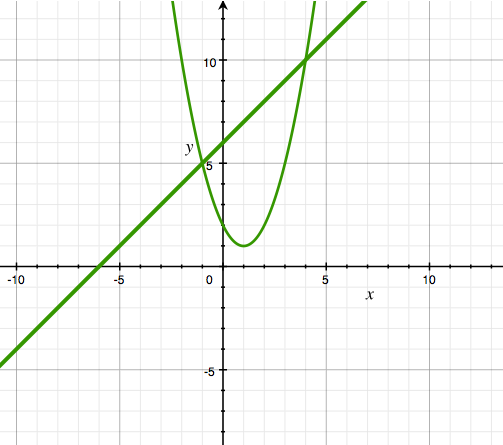
\includegraphics[width = 70mm]{images/231.png}
\end{center} 
Найдем точки пересечения этих функций: 
\begin{gather*}
x^2 - 2x + 2 = x + 6 \Rightarrow x^2 - 3x - 4 = 0 \Rightarrow x = 4, \; -1
\end{gather*}
Искомая площадь есть ни что иное, как разность площадей наших графиков между найденными точками, то есть интеграл разности:
\begin{gather*}
\int\limits_{-1}^4 ((x + 6) - (x^2 - 2x + 2))dx = 
\int\limits_{-1}^4 (-x^2 + 3x + 4)dx = 
(-\frac{x^3}3 + \frac{3x^2}{2} + 4x) \big |_{-1}^{4} = \frac{125}6   
\end{gather*}
\\ \\


%%%----------%%%----------%%%----------%%%----------%%%



\textbf{\large Задача 24}
\medskip\hrule\medskip
\textit{Найдите площадь фигуры, ограниченной линией, заданной в полярной системе координат указанным уравнением. Сделайте рисунок(6)}
\begin{align*}
\rho = 3 \cos 2\varphi
\end{align*}
\begin{center}
	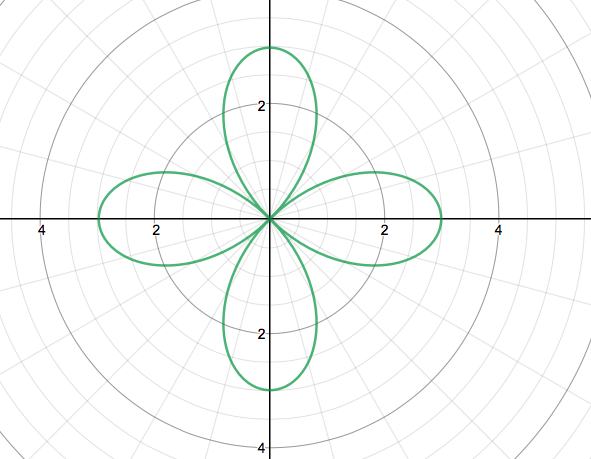
\includegraphics[width = 70mm]{images/241.png}
\end{center}
\begin{gather*}
S = \int\limits_{0}^{2\pi} \frac12 \rho^2 d\varphi = 
9\int\limits_{0}^{2\pi} \cos^2 (2\varphi)  d\varphi = 
9\int\limits_{0}^{2\pi} \frac{1 + \cos(4 \varphi)}2 d\varphi = 
\frac98\int\limits_{0}^{2\pi} (1 + \cos(4 \varphi)) d(4\varphi) = 
\begin{bmatrix} z = 4 \varphi \end{bmatrix} =\\[2pt]
\frac98\int\limits_{0}^{8\pi} (1 + \cos(z)) dz = 9\pi + \sin z \big |_{0}^{8\pi} = 9\pi
\end{gather*}
\newpage



%%%----------%%%----------%%%----------%%%----------%%%



\textbf{\large Задача 25}
\medskip\hrule\medskip
\textit{Найдите объем тела, образованного вращением вокруг оси $ Ox $ фигуры, ограниченной линией, заданной указанным уравнением(10)}
\begin{align*}
y = 2 \ln x + 3x \qquad 1 \leq x \leq 4 
\end{align*}
\begin{gather*}
V = \int\limits_{1}^{4} \pi y^2 dx =
\int\limits_{1}^{4} \pi (2 \ln x + 3x)^2 dx = 
\int\limits_{1}^{4} \pi (4 \ln^2x + 12 x\ln x + 9x^2)dx
\end{gather*}
Найдем сперва каждый из интегралов по отдельности
\begin{gather*}
\int \ln^2 x \; dx = 
x\ln^2 x - \int 2\ln x \; x \cdot dx/x + C = 
x\ln^2 x - \int 2\ln x\cdot dx + C = 
x\ln^2 - 2x\ln x  + 2 \int dx + C =\\[2pt] 
= x\ln^2 x - 2x\ln x + 2x + C\\[5pt]
\int x \ln x dx = \frac12 x^2 \ln x - \int \frac12xdx + C =
\frac12 x^2 \ln x - \frac14x^2 + C\\[5pt]
\end{gather*}
Теперь можем собрать все вместе:
\begin{gather*}
V = \int\limits_{1}^{4} \pi y^2 dx = 
\int\limits_{1}^{4} \pi (4 \ln^2x + 12 x\ln x + 9x^2)dx = 
\pi (4x\ln^2 x - 8x\ln x + 8x + 6x^2 \ln x - 3x^2 + 3x^3) \big |_{1}^{4} \approx\\
\approx 903.12
\end{gather*}
\\ \\ \\ 



%%%----------%%%----------%%%----------%%%----------%%%



\textbf{\large Задача 26}
\medskip\hrule\medskip
\textit{Найдите приблеженное значение интеграла с помощью методов а) прямоугольников б) трапеций в) Симпсона. При этом возьмите $ n = 10 $. Найдите верхние оценки погрешности вычислений.}
\begin{align*}
\int\limits_{1}^{3} \sqrt{16 + \sin^2(2x)} dx
\end{align*} \\
а) Метод прямоугольников 
\begin{gather*}
\int\limits_a^b f(x) dx = \sum_{i = 1}^{n} f(\frac{x_i + x_{i - 1}}{2})(x_i - x_{i - 1}) \\
E(f) = \frac{maxf''(x_i)(b - a)^3}{24n^2} \\[2pt]
f'' = \frac{d^2}{d^2x}(\sqrt{16 + \sin^2(2x)}) = -\frac{(4 sin^2(2 x))}{\sqrt{\sin^2(2 x) + 16}} + \frac{(4 \cos^2(2 x))}{\sqrt{\sin^2(2 x) + 16}} - \frac{(4 \sin^2(2 x) \cos^2(2 x))}{(\sin^2(2 x) + 16)^{\frac32}} 
\end{gather*}
\begin{center}
	\begin{tabular}{|c|c|c|c|}
		\hline
		 $ n $ & $ x $ & $ f(\frac{x_i + x_{i - 1}}2) $ & $ f'' $ \\[2pt]
		\hline
		$ 0 $  &   $ 1.0 $   &   $ 4.081 $   &  -0.65 \\[2pt]
		\hline
		$ 1 $  &   $ 1.2 $   &   $ 4.033 $   &  0.071 \\[2pt]
		\hline
		$ 2 $  &   $ 1.4 $   &   $ 4.002 $   &  0.767 \\[2pt]
		\hline
		$ 3 $  &   $ 1.6 $   &   $ 4.008 $   &   0.993 \\[2pt]
		\hline
		$ 4 $  &   $ 1.8 $   &   $ 4.047 $   &  0.595 \\[2pt]
		\hline
		$ 5 $  &   $ 2.0 $   &   $ 4.094 $   &   -0.157 \\[2pt]
		\hline
		$ 6 $  &   $ 2.2 $   &   $ 4.122 $   &  -0.793 \\[2pt]
		\hline
		$ 7 $  &   $ 2.4 $   &   $ 4.113 $   &  -0.956 \\[2pt]
		\hline
		$ 8 $  &   $ 2.6 $   &   $ 4.074 $   &  -0.558 \\[2pt]
		\hline
		$ 9 $  &   $ 2.8 $   &   $ 4.027 $   &   0.186 \\[2pt]
		\hline
		$ 10 $  &   $ 3.0 $   &   $ 4.001 $   &  0.837 \\[2pt]
		\hline
	\end{tabular}
\end{center}
\begin{gather*}
 \sum_{i = 1}^{n} f(\frac{x_i + x_{i - 1}}{2})(x_i - x_{i - 1}) \approx 8.920 \\
 E(f) = \frac{0.956 \cdot 2^3}{24 \cdot 100} = 0.003
\end{gather*}
б) Метод трапеций
\begin{gather*}
\int\limits_a^b f(x) dx = \sum_{i = 1}^{n} \frac{f(x_i) + f(x_{i - 1})}2 \cdot \frac{(b - a)}{n} \\
E(f) = \frac{maxf''(x_i)(b - a)^3}{12n^2} \\[2pt]
\end{gather*}
\begin{center}
	\begin{tabular}{|c|c|c|}
		\hline
		$ n $ & $ x $ & $ \frac{f(x_i) + f(x_{i - 1})}2 $ \\[2pt]
		\hline
		$ 0 $  &   $ 1.0 $   &   $ 4.113 $  \\[2pt]
		\hline
		$ 1 $  &   $ 1.2 $   &   $ 4.079 $     \\[2pt]
		\hline
		$ 2 $  &   $ 1.4 $   &   $ 4.035 $     \\[2pt]
		\hline
		$ 3 $  &   $ 1.6 $   &   $ 4.007 $      \\[2pt]
		\hline
		$ 4 $  &   $ 1.8 $   &   $ 4.012 $      \\[2pt]
		\hline
		$ 5 $  &   $ 2.0 $   &   $ 4.048 $      \\[2pt]
		\hline
		$ 6 $  &   $ 2.2 $   &   $ 4.091 $      \\[2pt]
		\hline
		$ 7 $  &   $ 2.4 $   &   $ 4.117 $      \\[2pt]
		\hline
		$ 8 $  &   $ 2.6 $   &   $ 4.109 $      \\[2pt]
		\hline
		$ 9 $  &   $ 2.8 $   &   $ 4.073 $      \\[2pt]
		\hline
		$ 10 $  &   $ 3.0 $   &   $ 4.03 $      \\[2pt]
		\hline
	\end{tabular}
\end{center}
\begin{gather*}
\sum_{i = 1}^{n} \frac{f(x_i) + f(x_{i - 1})}2 \cdot \frac{(b - a)}{n} \approx 8.943 \\
E(f) = \frac{0.956 \cdot 2^3}{12 \cdot 100} = 0.006
\end{gather*}
в) Метод Симпсона
\begin{gather*}
\int\limits_a^b f(x) dx = \sum_{i = 1}^{n} \frac{f(x_{i - 1}) + 4f(\frac{x_{i - 1} + x_i}2)) + f(x_i)}{6} \cdot \frac{b - a}{n} \\[2pt]
E(f) = \frac{maxf^{(4)}(x_i)(b - a)^5}{2880} \\[2pt]
\end{gather*}
\begin{center}
	\begin{tabular}{|c|c|c|}
		\hline
		$ n $ & $ x $ & $ \frac{f(x_{i - 1}) + 4f(\frac{x_{i - 1} + x_i}2)) + f(x_i)}{6} $ \\[3pt]
		\hline
		$ 0 $  &   $ 1.0 $   &   $ 4.08 $     \\[2pt]
		\hline
		$ 1 $  &   $ 1.2 $   &   $ 4.034 $     \\[2pt]
		\hline
		$ 2 $  &   $ 1.4 $   &   $ 4.004 $     \\[2pt]
		\hline
		$ 3 $  &   $ 1.6 $   &   $ 4.01 $     \\[2pt]
		\hline
		$ 4 $  &   $ 1.8 $   &   $ 4.047 $     \\[2pt]
		\hline
		$ 5 $  &   $ 2.0 $   &   $ 4.093 $     \\[2pt]
		\hline
		$ 6 $  &   $ 2.2 $   &   $ 4.12 $     \\[2pt]
		\hline
		$ 7 $  &   $ 2.4 $   &   $ 4.112 $     \\[2pt]
		\hline
		$ 8 $  &   $ 2.6 $   &   $ 4.074 $     \\[2pt]
		\hline
		$ 9 $  &   $ 2.8 $   &   $ 4.028 $     \\[2pt]
		\hline
		$ 10 $  &   $ 3.0 $   &   $ 4.002 $     \\[2pt]
		\hline
	\end{tabular}
\end{center}
\begin{gather*}
\sum_{i = 1}^{n} \frac{f(x_{i - 1}) + 4f(\frac{x_{i - 1} + x_i}2)) + f(x_i)}{6} \cdot \frac{b - a}{n} \approx 8.921
\end{gather*}
Оценим производную 4 порядка с помощью Wolphram Alpha:
$ f^{(4)} \approx 3.191 $ \\
\begin{center}
	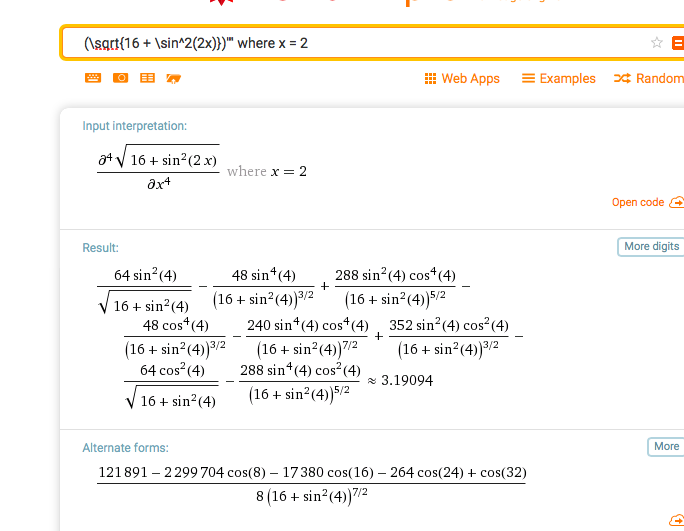
\includegraphics[width = 50mm]{images/261.png}
\end{center}
\begin{gather*}
E(f) = \frac{maxf^{(4)}(x_i)(b - a)^5}{2880}  = \frac{3.191 \cdot 2^5}{2880} \approx 0.035
\end{gather*}
\end{document}